\documentclass[11pt]{article}
\usepackage[textwidth=18.0cm, textheight=23.0cm, top=2.0cm]{geometry}
\usepackage{pst-all}
\usepackage{amssymb}
\usepackage{tikz}
\usepackage{underscore}\begin{document}
\pagestyle{empty}


ClassName: \underline{\textbf{Class_08.2bp-35}}
\par
BinSize: \underline{\textbf{100 × 100}}
\par
ReduceSize: \underline{\textbf{100 × 100}}
\par
TypeNum: \underline{\textbf{79}}
\par
Num: \underline{\textbf{80}}
\par
OutS: \underline{\textbf{220000}}
\par
InS: \underline{\textbf{187151}}
\par
Rate: \underline{\textbf{0.851}}
\par
UB: \underline{\textbf{22}}
\par
LB0: \underline{\textbf{22}}
\par
LB: \underline{\textbf{22}}
\par
LBWithCut: \underline{\textbf{22}}
\par
NodeCut: \underline{\textbf{0}}
\par
ExtendedNodeCnt: \underline{\textbf{1}}
\par
GenNodeCnt: \underline{\textbf{1}}
\par
PrimalNode: \underline{\textbf{0}}
\par
ColumnCount: \underline{\textbf{22}}
\par
TotalCutCount: \underline{\textbf{0}}
\par
RootCutCount: \underline{\textbf{0}}
\par
LPSolverCnt: \underline{\textbf{1}}
\par
PricingSolverCnt: \underline{\textbf{0}}
\par
BranchAndBoundNum: \underline{\textbf{1}}
\par
isOpt: \underline{\textbf{true}}
\par
TimeOnInitSolution: \underline{\textbf{0.220 s}}
\par
TimeOnPrimal: \underline{\textbf{0.000 s}}
\par
TimeOnPricing: \underline{\textbf{0.000 s}}
\par
TimeOnRmp: \underline{\textbf{0.078 s}}
\par
TotalTime: \underline{\textbf{0.345 s}}
\par
\newpage


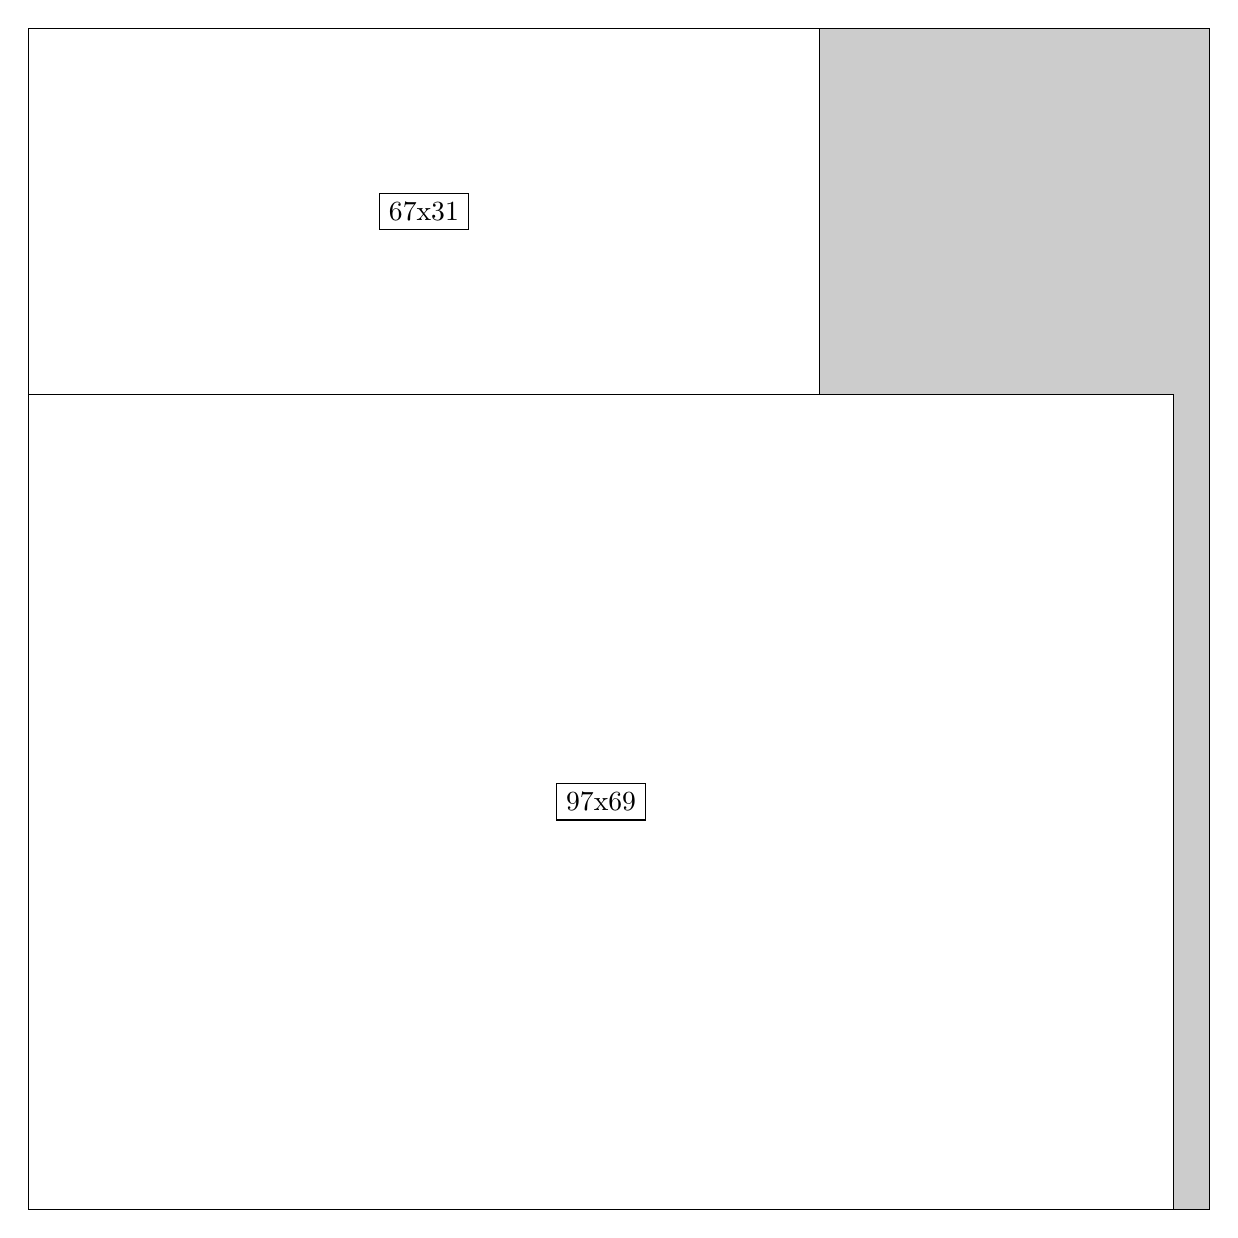
\begin{tikzpicture}[shorten >=1pt,scale=1.0,every node/.style={scale=1.0},->]
\tikzstyle{vertex}=[circle,fill=black!25,minimum size=14pt,inner sep=0pt]
\filldraw[fill=gray!40!white, draw=black] (0,0) rectangle (15.0,15.0);
\foreach \name/\x/\y/\w/\h in {97x69/0.0/0.0/14.549999999999999/10.35,67x31/0.0/10.35/10.049999999999999/4.6499999999999995}
\filldraw[fill=white!40!white, draw=black] (\x,\y) rectangle node[draw] (\name) {\name} ++(\w,\h);
\end{tikzpicture}


w =97 , h =69 , x =0 , y =0 , v =6693
\par
w =67 , h =31 , x =0 , y =69 , v =2077
\par
\newpage


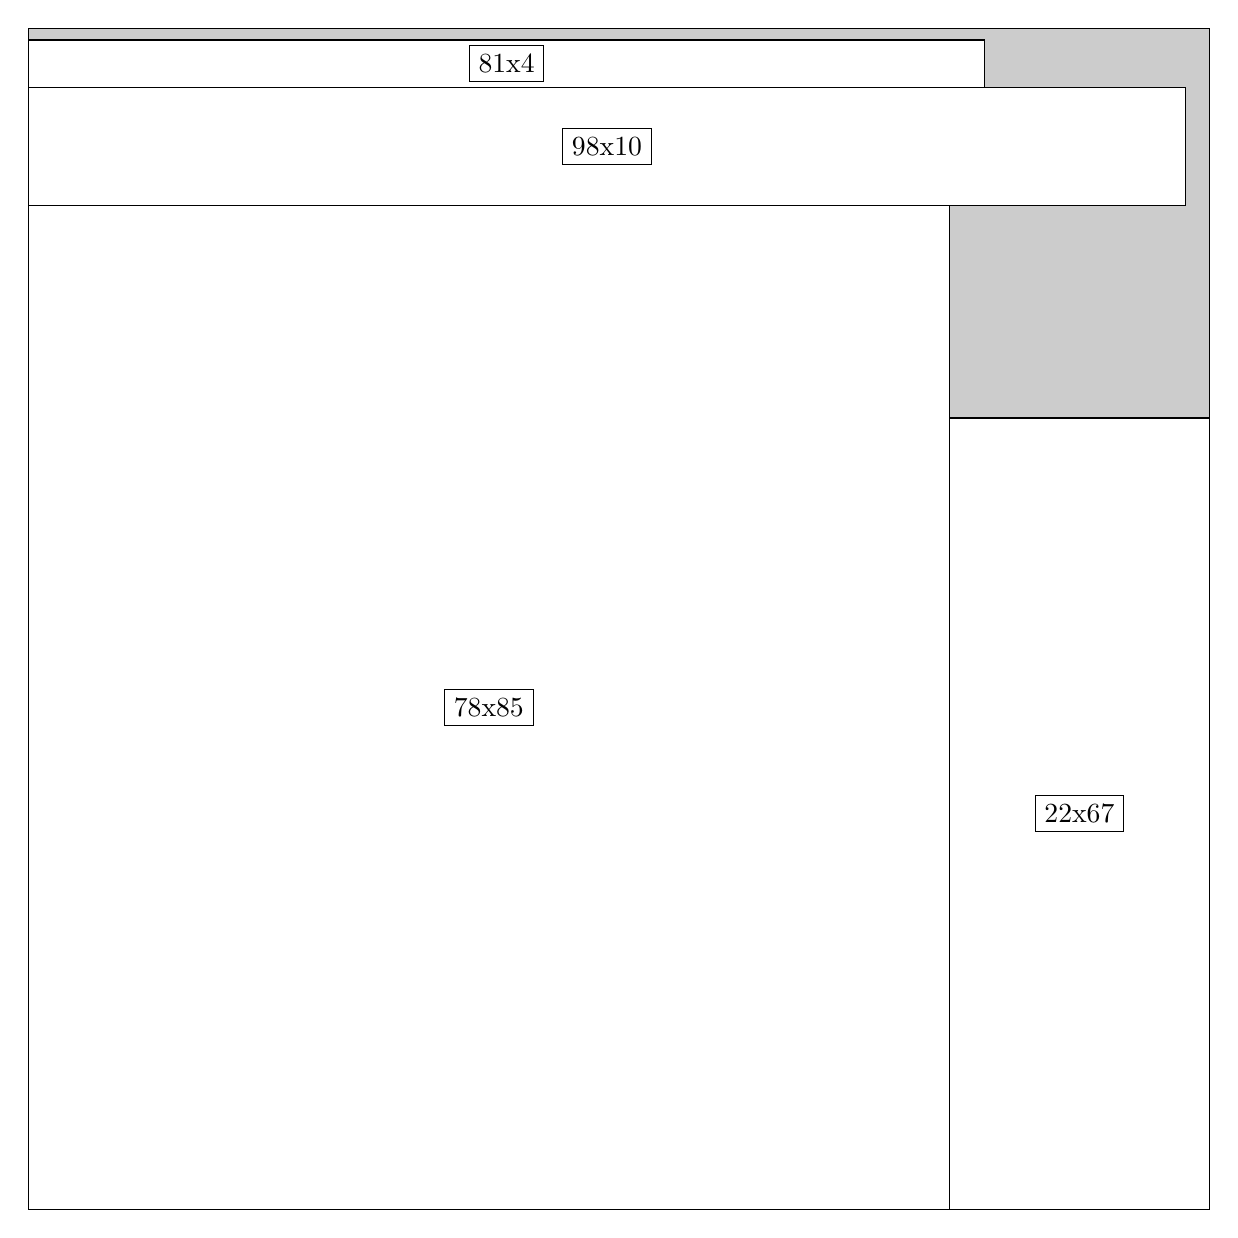
\begin{tikzpicture}[shorten >=1pt,scale=1.0,every node/.style={scale=1.0},->]
\tikzstyle{vertex}=[circle,fill=black!25,minimum size=14pt,inner sep=0pt]
\filldraw[fill=gray!40!white, draw=black] (0,0) rectangle (15.0,15.0);
\foreach \name/\x/\y/\w/\h in {78x85/0.0/0.0/11.7/12.75,22x67/11.7/0.0/3.3/10.049999999999999,98x10/0.0/12.75/14.7/1.5,81x4/0.0/14.25/12.15/0.6}
\filldraw[fill=white!40!white, draw=black] (\x,\y) rectangle node[draw] (\name) {\name} ++(\w,\h);
\end{tikzpicture}


w =78 , h =85 , x =0 , y =0 , v =6630
\par
w =22 , h =67 , x =78 , y =0 , v =1474
\par
w =98 , h =10 , x =0 , y =85 , v =980
\par
w =81 , h =4 , x =0 , y =95 , v =324
\par
\newpage


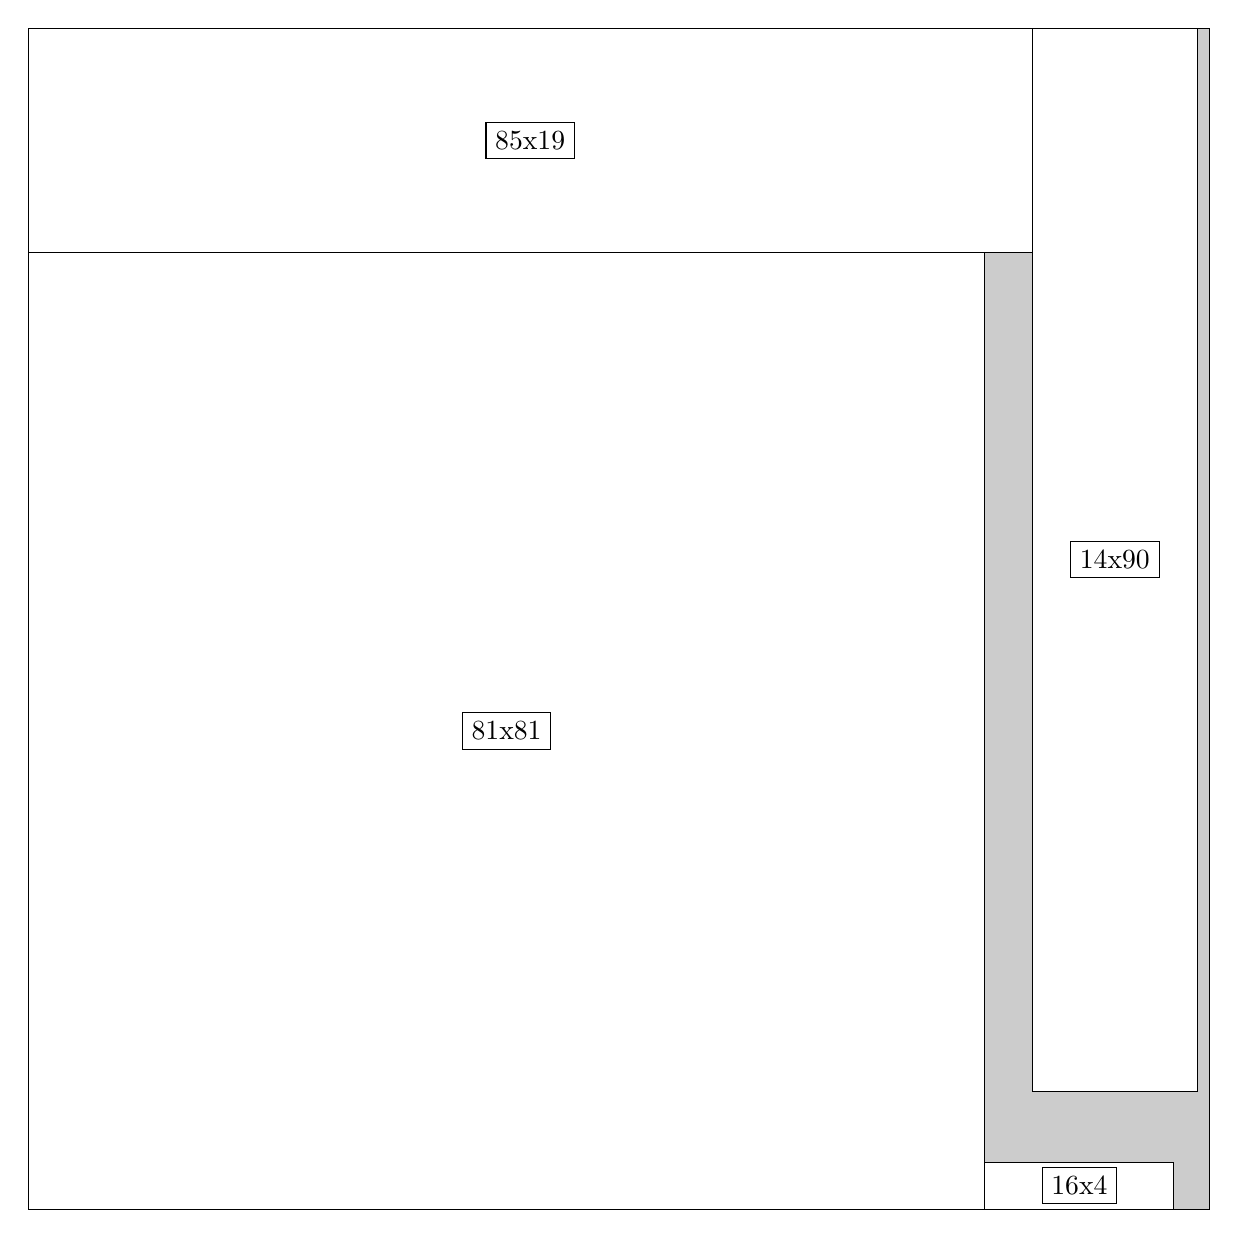
\begin{tikzpicture}[shorten >=1pt,scale=1.0,every node/.style={scale=1.0},->]
\tikzstyle{vertex}=[circle,fill=black!25,minimum size=14pt,inner sep=0pt]
\filldraw[fill=gray!40!white, draw=black] (0,0) rectangle (15.0,15.0);
\foreach \name/\x/\y/\w/\h in {81x81/0.0/0.0/12.15/12.15,85x19/0.0/12.15/12.75/2.85,14x90/12.75/1.5/2.1/13.5,16x4/12.15/0.0/2.4/0.6}
\filldraw[fill=white!40!white, draw=black] (\x,\y) rectangle node[draw] (\name) {\name} ++(\w,\h);
\end{tikzpicture}


w =81 , h =81 , x =0 , y =0 , v =6561
\par
w =85 , h =19 , x =0 , y =81 , v =1615
\par
w =14 , h =90 , x =85 , y =10 , v =1260
\par
w =16 , h =4 , x =81 , y =0 , v =64
\par
\newpage


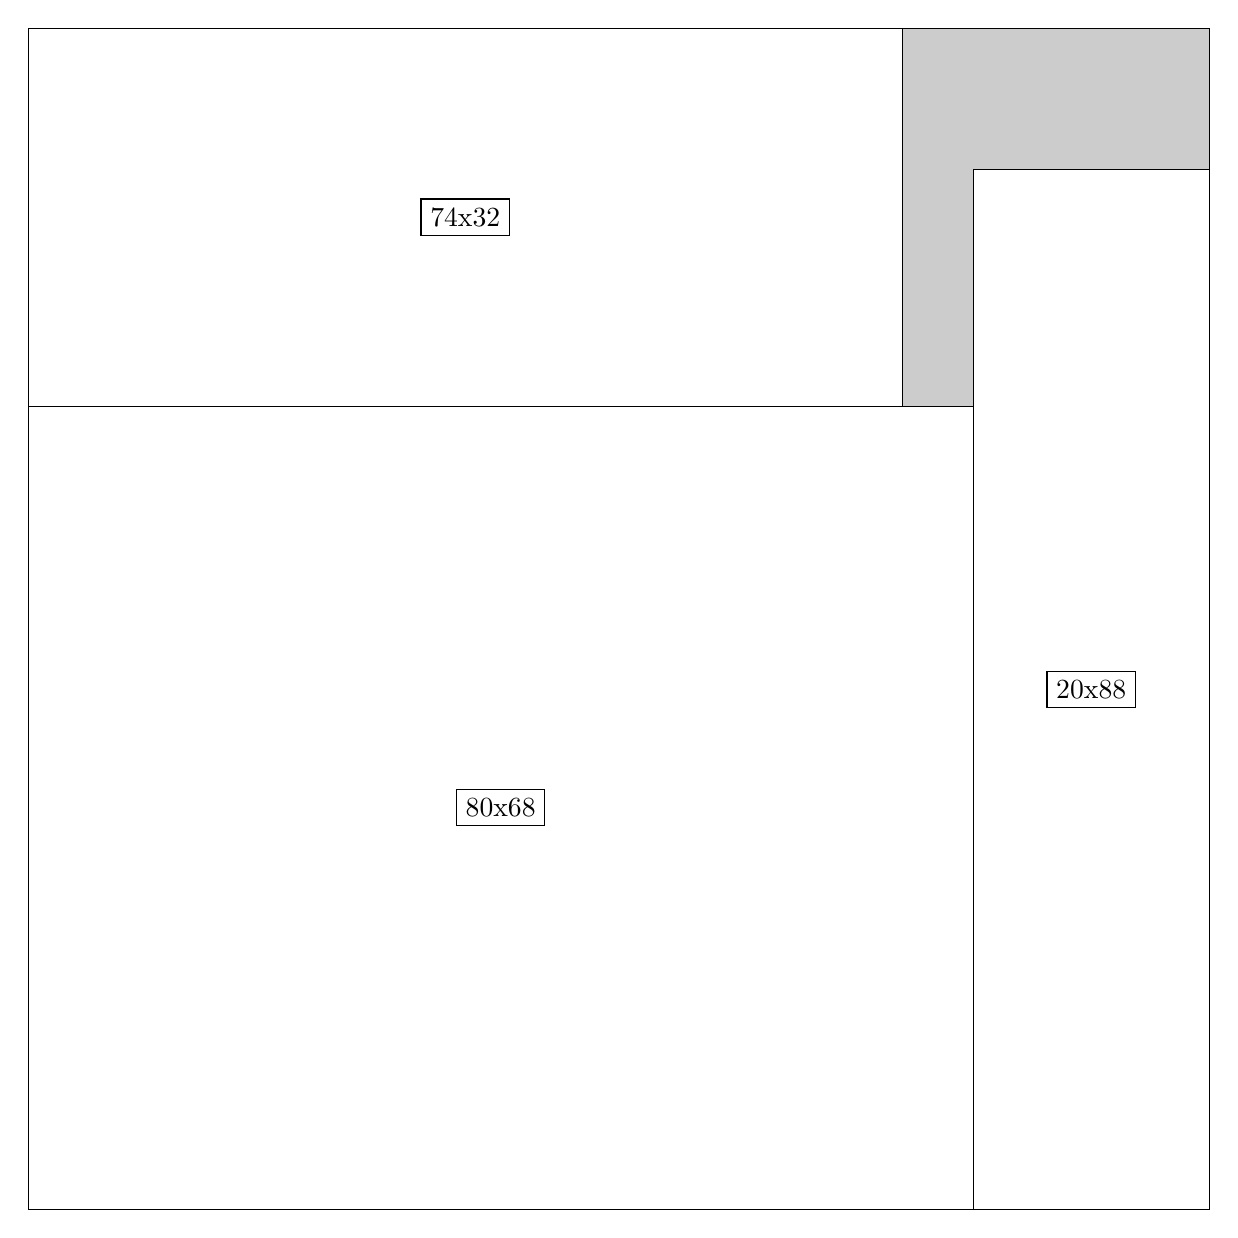
\begin{tikzpicture}[shorten >=1pt,scale=1.0,every node/.style={scale=1.0},->]
\tikzstyle{vertex}=[circle,fill=black!25,minimum size=14pt,inner sep=0pt]
\filldraw[fill=gray!40!white, draw=black] (0,0) rectangle (15.0,15.0);
\foreach \name/\x/\y/\w/\h in {80x68/0.0/0.0/12.0/10.2,74x32/0.0/10.2/11.1/4.8,20x88/12.0/0.0/3.0/13.2}
\filldraw[fill=white!40!white, draw=black] (\x,\y) rectangle node[draw] (\name) {\name} ++(\w,\h);
\end{tikzpicture}


w =80 , h =68 , x =0 , y =0 , v =5440
\par
w =74 , h =32 , x =0 , y =68 , v =2368
\par
w =20 , h =88 , x =80 , y =0 , v =1760
\par
\newpage


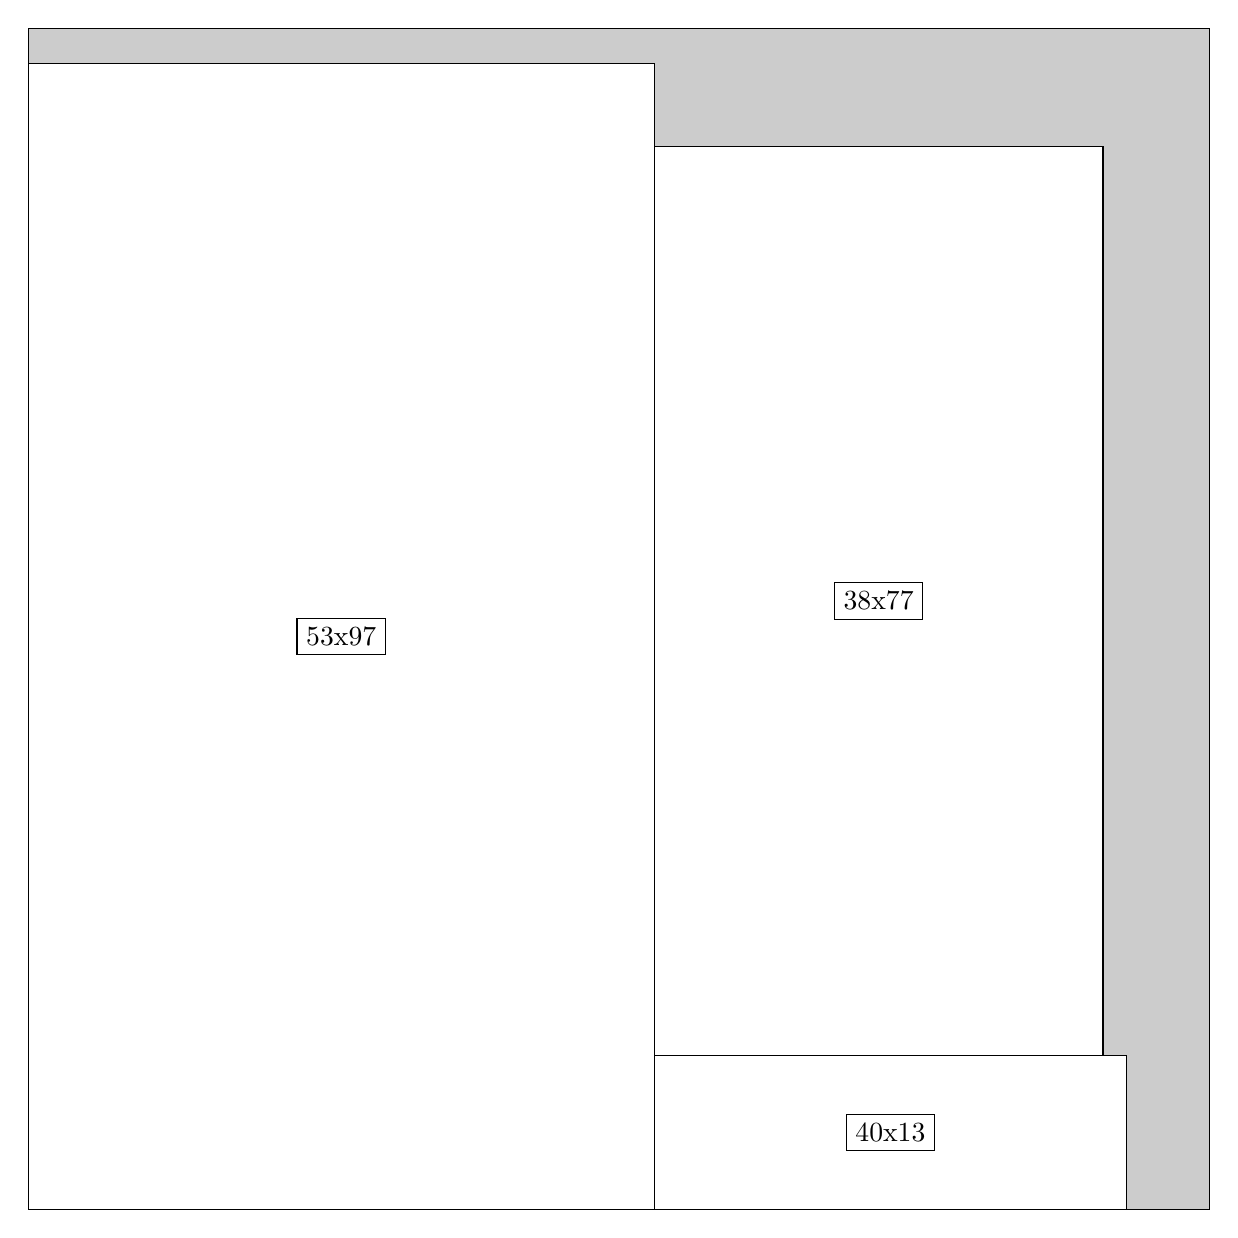
\begin{tikzpicture}[shorten >=1pt,scale=1.0,every node/.style={scale=1.0},->]
\tikzstyle{vertex}=[circle,fill=black!25,minimum size=14pt,inner sep=0pt]
\filldraw[fill=gray!40!white, draw=black] (0,0) rectangle (15.0,15.0);
\foreach \name/\x/\y/\w/\h in {53x97/0.0/0.0/7.949999999999999/14.549999999999999,38x77/7.949999999999999/1.95/5.7/11.549999999999999,40x13/7.949999999999999/0.0/6.0/1.95}
\filldraw[fill=white!40!white, draw=black] (\x,\y) rectangle node[draw] (\name) {\name} ++(\w,\h);
\end{tikzpicture}


w =53 , h =97 , x =0 , y =0 , v =5141
\par
w =38 , h =77 , x =53 , y =13 , v =2926
\par
w =40 , h =13 , x =53 , y =0 , v =520
\par
\newpage


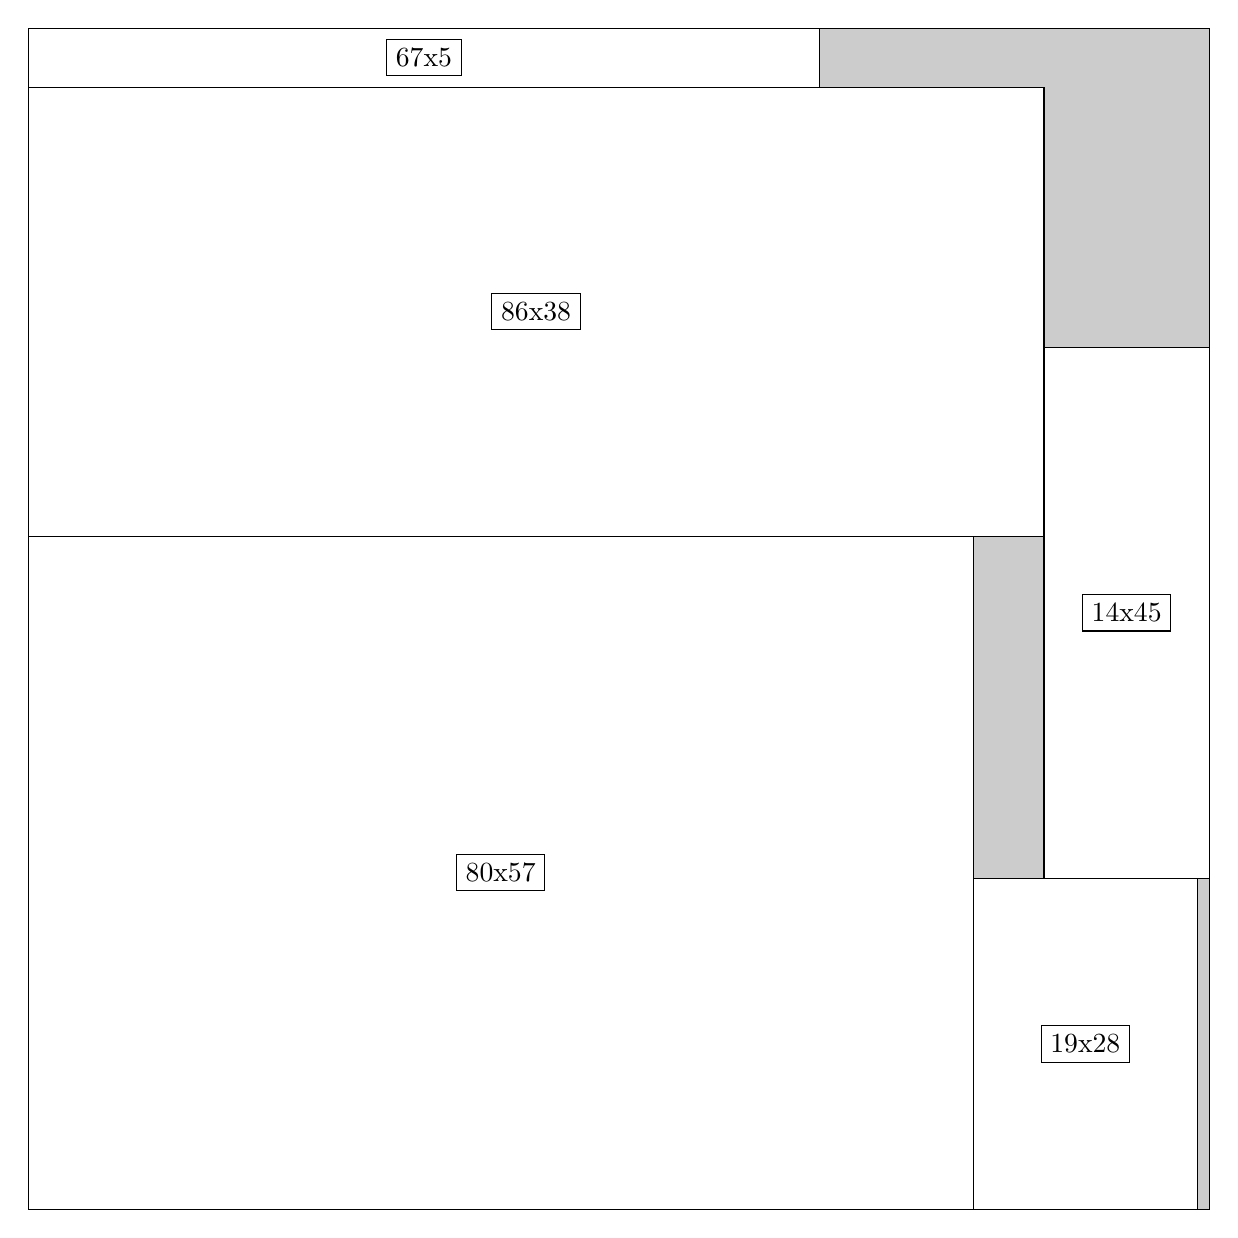
\begin{tikzpicture}[shorten >=1pt,scale=1.0,every node/.style={scale=1.0},->]
\tikzstyle{vertex}=[circle,fill=black!25,minimum size=14pt,inner sep=0pt]
\filldraw[fill=gray!40!white, draw=black] (0,0) rectangle (15.0,15.0);
\foreach \name/\x/\y/\w/\h in {80x57/0.0/0.0/12.0/8.549999999999999,67x5/0.0/14.25/10.049999999999999/0.75,86x38/0.0/8.549999999999999/12.9/5.7,14x45/12.9/4.2/2.1/6.75,19x28/12.0/0.0/2.85/4.2}
\filldraw[fill=white!40!white, draw=black] (\x,\y) rectangle node[draw] (\name) {\name} ++(\w,\h);
\end{tikzpicture}


w =80 , h =57 , x =0 , y =0 , v =4560
\par
w =67 , h =5 , x =0 , y =95 , v =335
\par
w =86 , h =38 , x =0 , y =57 , v =3268
\par
w =14 , h =45 , x =86 , y =28 , v =630
\par
w =19 , h =28 , x =80 , y =0 , v =532
\par
\newpage


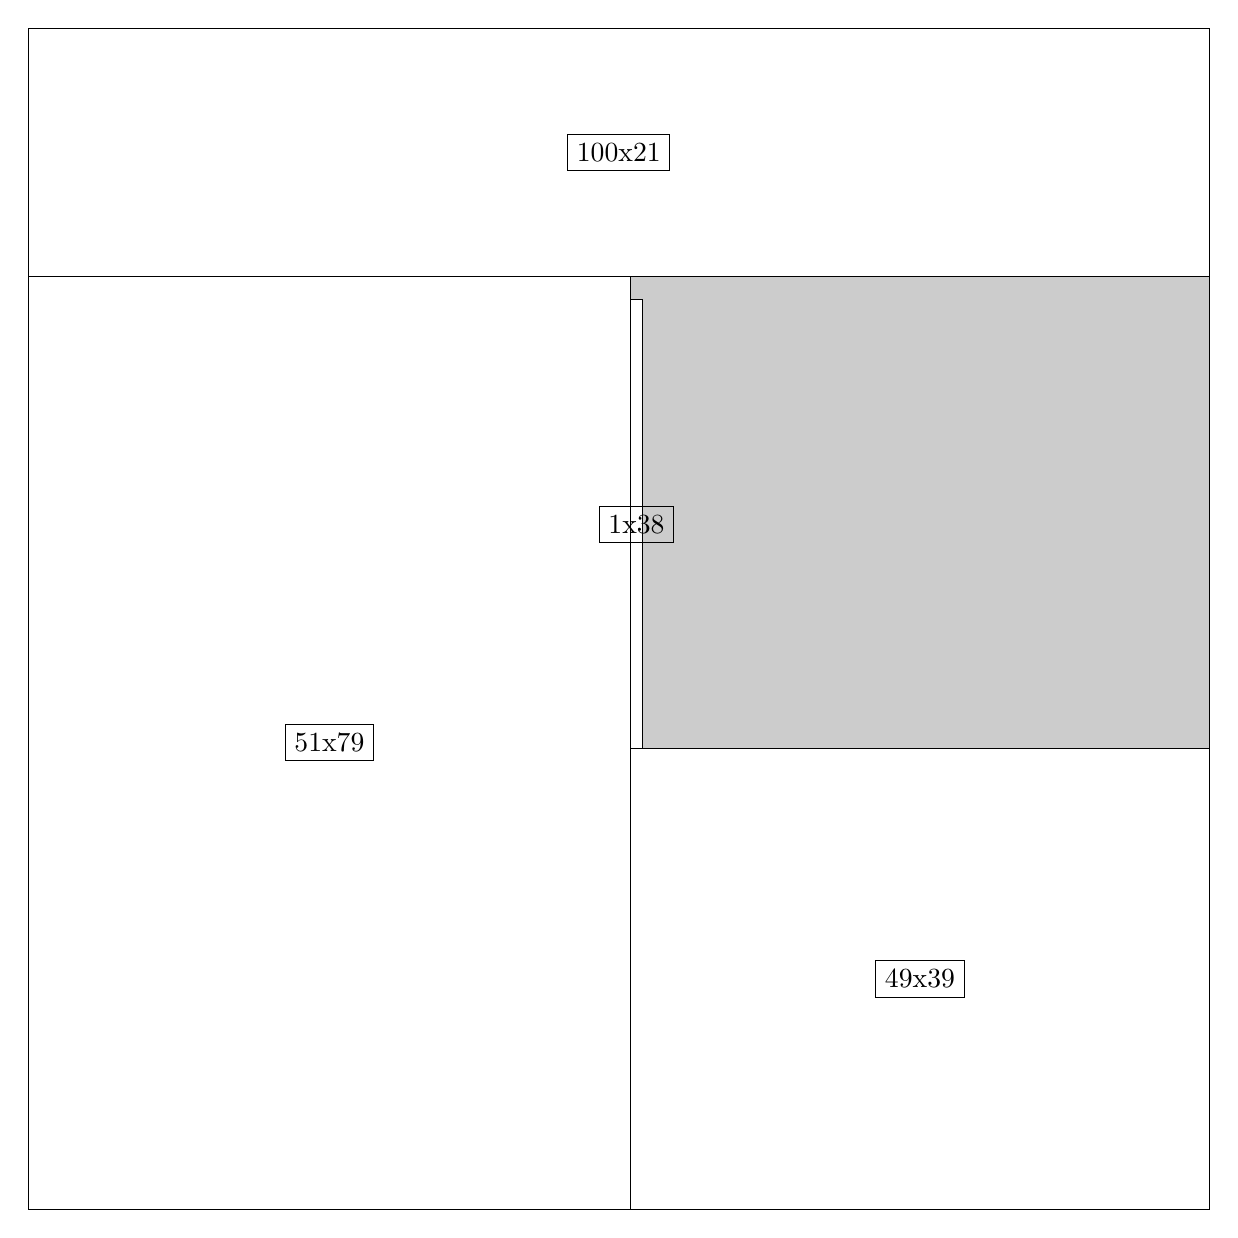
\begin{tikzpicture}[shorten >=1pt,scale=1.0,every node/.style={scale=1.0},->]
\tikzstyle{vertex}=[circle,fill=black!25,minimum size=14pt,inner sep=0pt]
\filldraw[fill=gray!40!white, draw=black] (0,0) rectangle (15.0,15.0);
\foreach \name/\x/\y/\w/\h in {51x79/0.0/0.0/7.6499999999999995/11.85,100x21/0.0/11.85/15.0/3.15,49x39/7.6499999999999995/0.0/7.35/5.85,1x38/7.6499999999999995/5.85/0.15/5.7}
\filldraw[fill=white!40!white, draw=black] (\x,\y) rectangle node[draw] (\name) {\name} ++(\w,\h);
\end{tikzpicture}


w =51 , h =79 , x =0 , y =0 , v =4029
\par
w =100 , h =21 , x =0 , y =79 , v =2100
\par
w =49 , h =39 , x =51 , y =0 , v =1911
\par
w =1 , h =38 , x =51 , y =39 , v =38
\par
\newpage


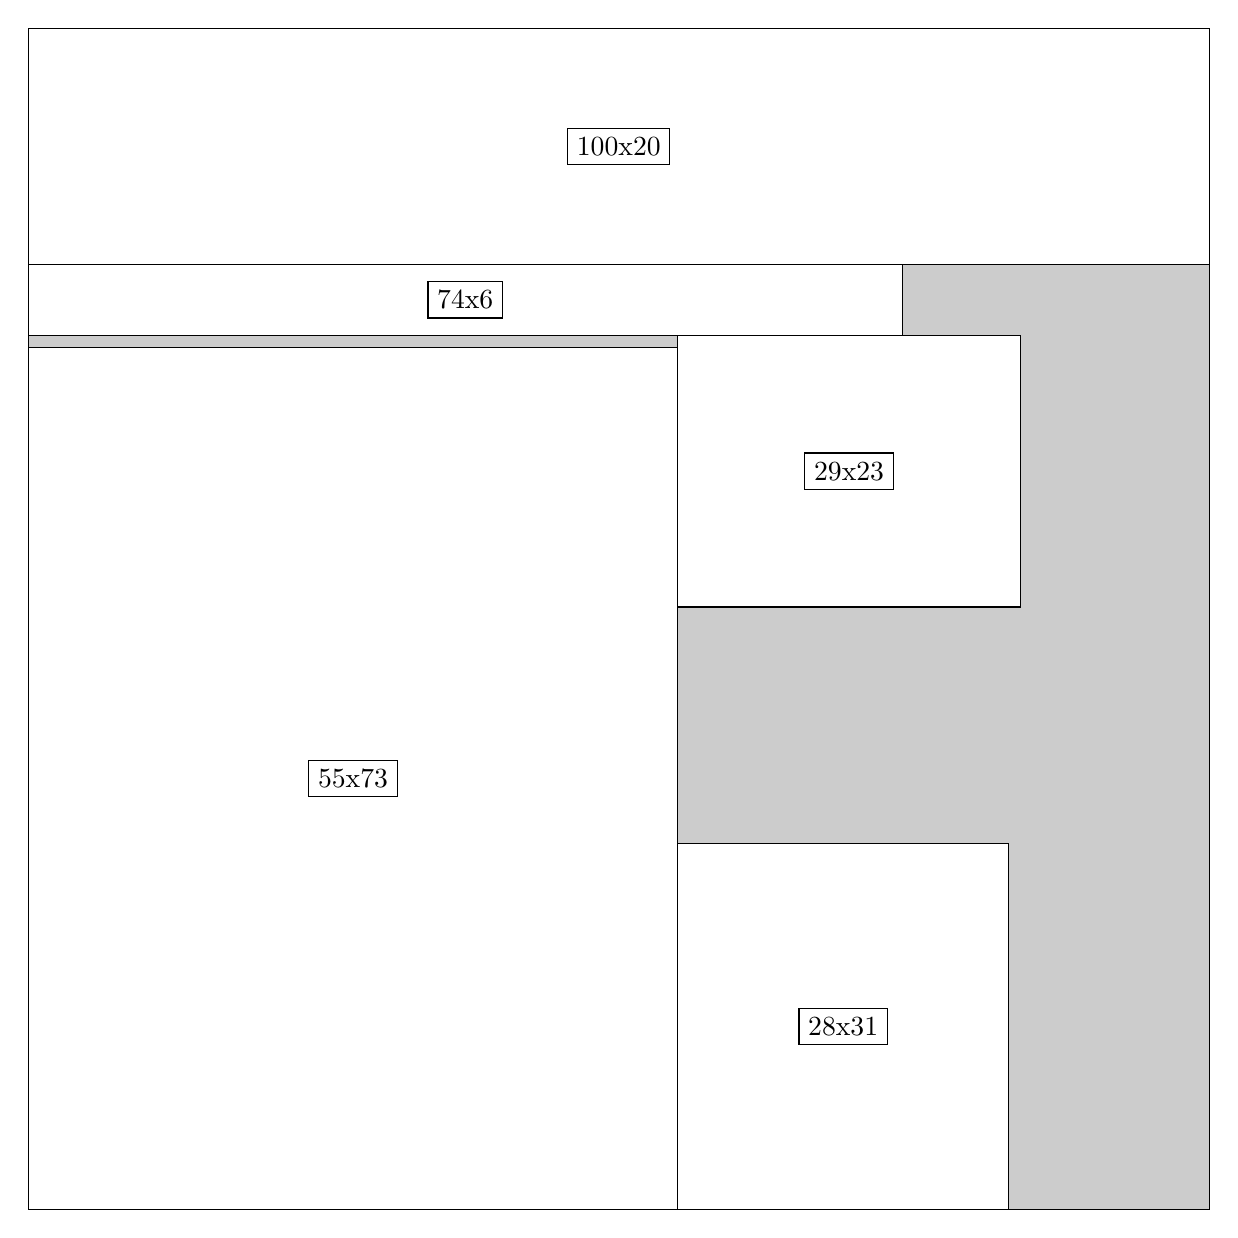
\begin{tikzpicture}[shorten >=1pt,scale=1.0,every node/.style={scale=1.0},->]
\tikzstyle{vertex}=[circle,fill=black!25,minimum size=14pt,inner sep=0pt]
\filldraw[fill=gray!40!white, draw=black] (0,0) rectangle (15.0,15.0);
\foreach \name/\x/\y/\w/\h in {55x73/0.0/0.0/8.25/10.95,100x20/0.0/12.0/15.0/3.0,28x31/8.25/0.0/4.2/4.6499999999999995,29x23/8.25/7.6499999999999995/4.35/3.4499999999999997,74x6/0.0/11.1/11.1/0.8999999999999999}
\filldraw[fill=white!40!white, draw=black] (\x,\y) rectangle node[draw] (\name) {\name} ++(\w,\h);
\end{tikzpicture}


w =55 , h =73 , x =0 , y =0 , v =4015
\par
w =100 , h =20 , x =0 , y =80 , v =2000
\par
w =28 , h =31 , x =55 , y =0 , v =868
\par
w =29 , h =23 , x =55 , y =51 , v =667
\par
w =74 , h =6 , x =0 , y =74 , v =444
\par
\newpage


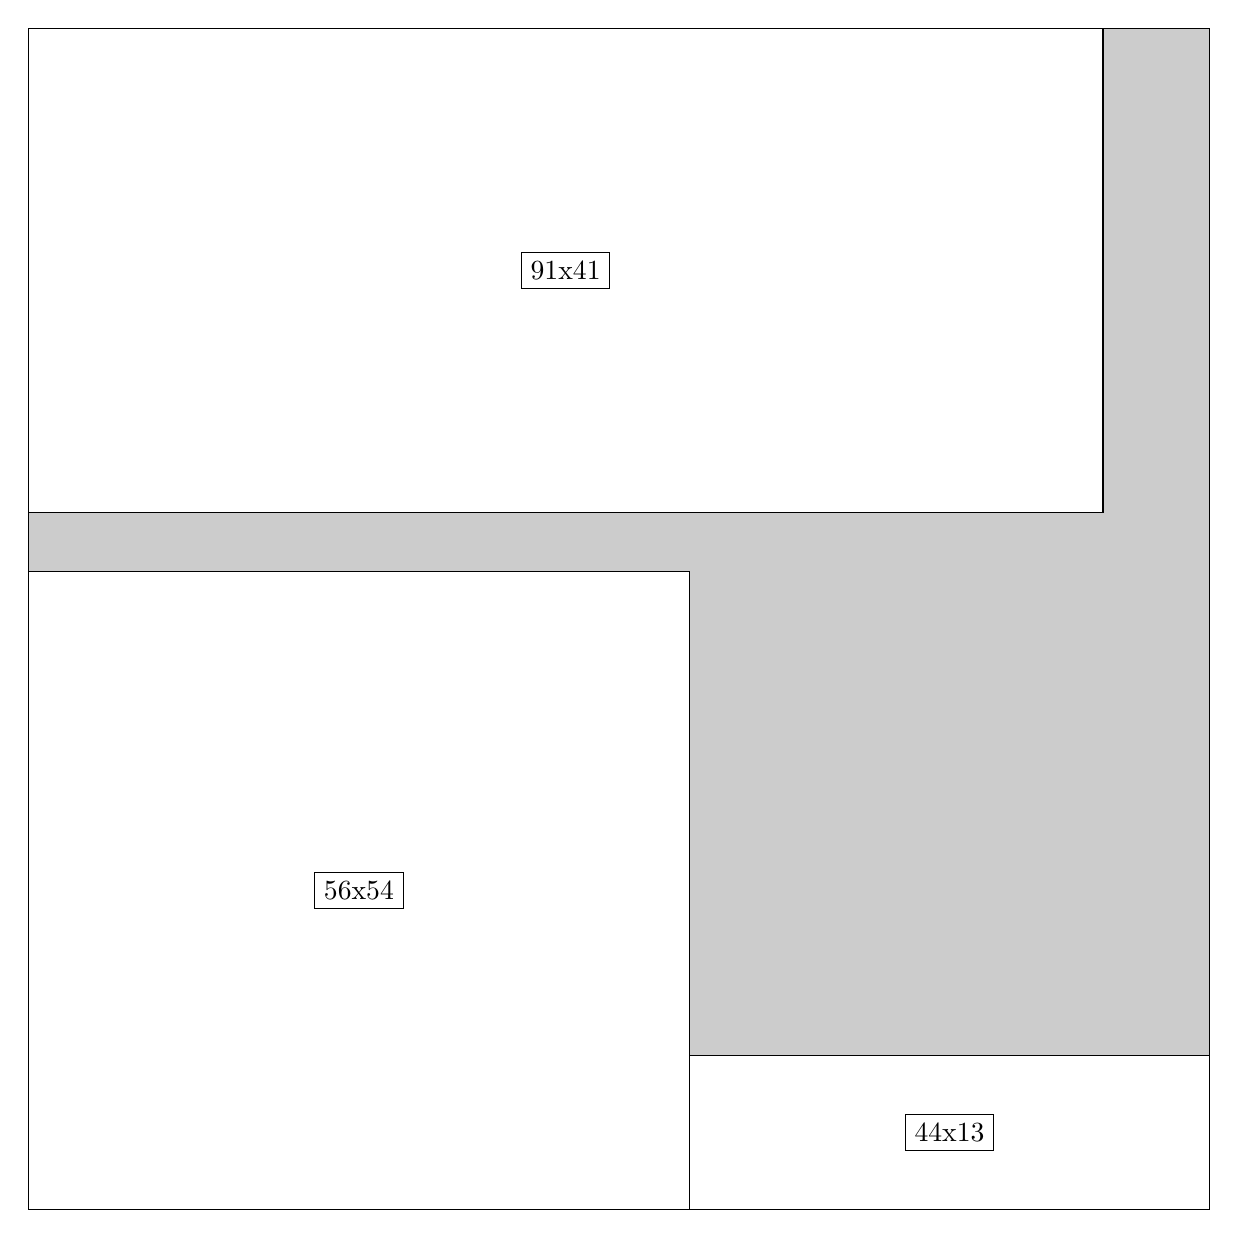
\begin{tikzpicture}[shorten >=1pt,scale=1.0,every node/.style={scale=1.0},->]
\tikzstyle{vertex}=[circle,fill=black!25,minimum size=14pt,inner sep=0pt]
\filldraw[fill=gray!40!white, draw=black] (0,0) rectangle (15.0,15.0);
\foreach \name/\x/\y/\w/\h in {91x41/0.0/8.85/13.65/6.1499999999999995,56x54/0.0/0.0/8.4/8.1,44x13/8.4/0.0/6.6/1.95}
\filldraw[fill=white!40!white, draw=black] (\x,\y) rectangle node[draw] (\name) {\name} ++(\w,\h);
\end{tikzpicture}


w =91 , h =41 , x =0 , y =59 , v =3731
\par
w =56 , h =54 , x =0 , y =0 , v =3024
\par
w =44 , h =13 , x =56 , y =0 , v =572
\par
\newpage


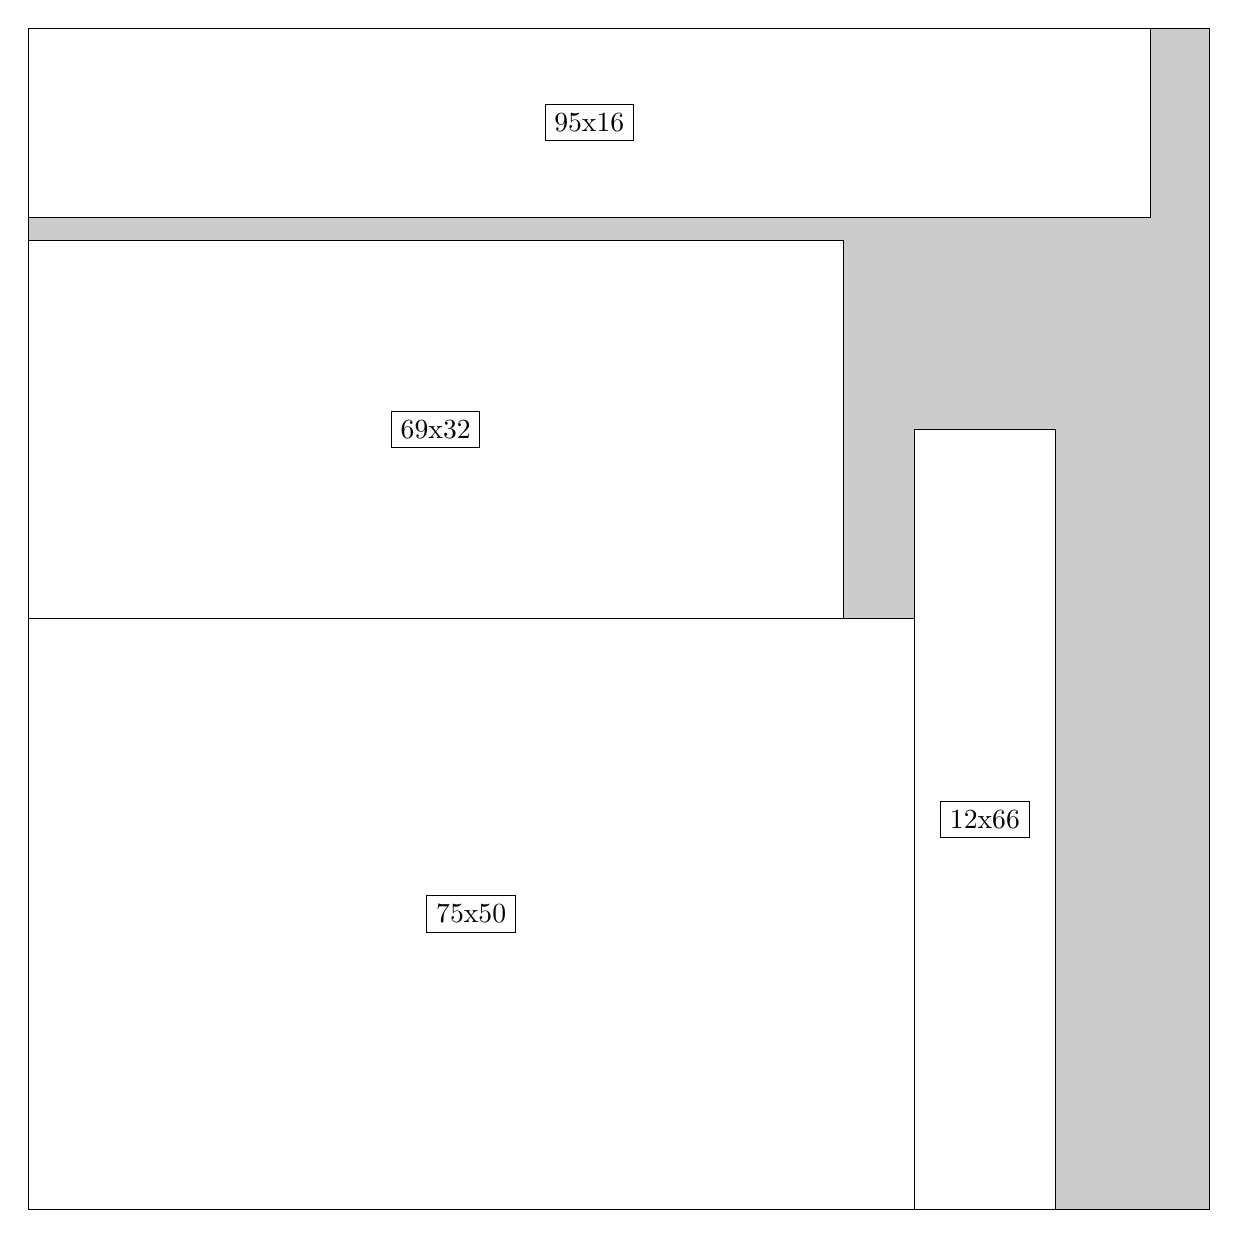
\begin{tikzpicture}[shorten >=1pt,scale=1.0,every node/.style={scale=1.0},->]
\tikzstyle{vertex}=[circle,fill=black!25,minimum size=14pt,inner sep=0pt]
\filldraw[fill=gray!40!white, draw=black] (0,0) rectangle (15.0,15.0);
\foreach \name/\x/\y/\w/\h in {75x50/0.0/0.0/11.25/7.5,95x16/0.0/12.6/14.25/2.4,69x32/0.0/7.5/10.35/4.8,12x66/11.25/0.0/1.7999999999999998/9.9}
\filldraw[fill=white!40!white, draw=black] (\x,\y) rectangle node[draw] (\name) {\name} ++(\w,\h);
\end{tikzpicture}


w =75 , h =50 , x =0 , y =0 , v =3750
\par
w =95 , h =16 , x =0 , y =84 , v =1520
\par
w =69 , h =32 , x =0 , y =50 , v =2208
\par
w =12 , h =66 , x =75 , y =0 , v =792
\par
\newpage


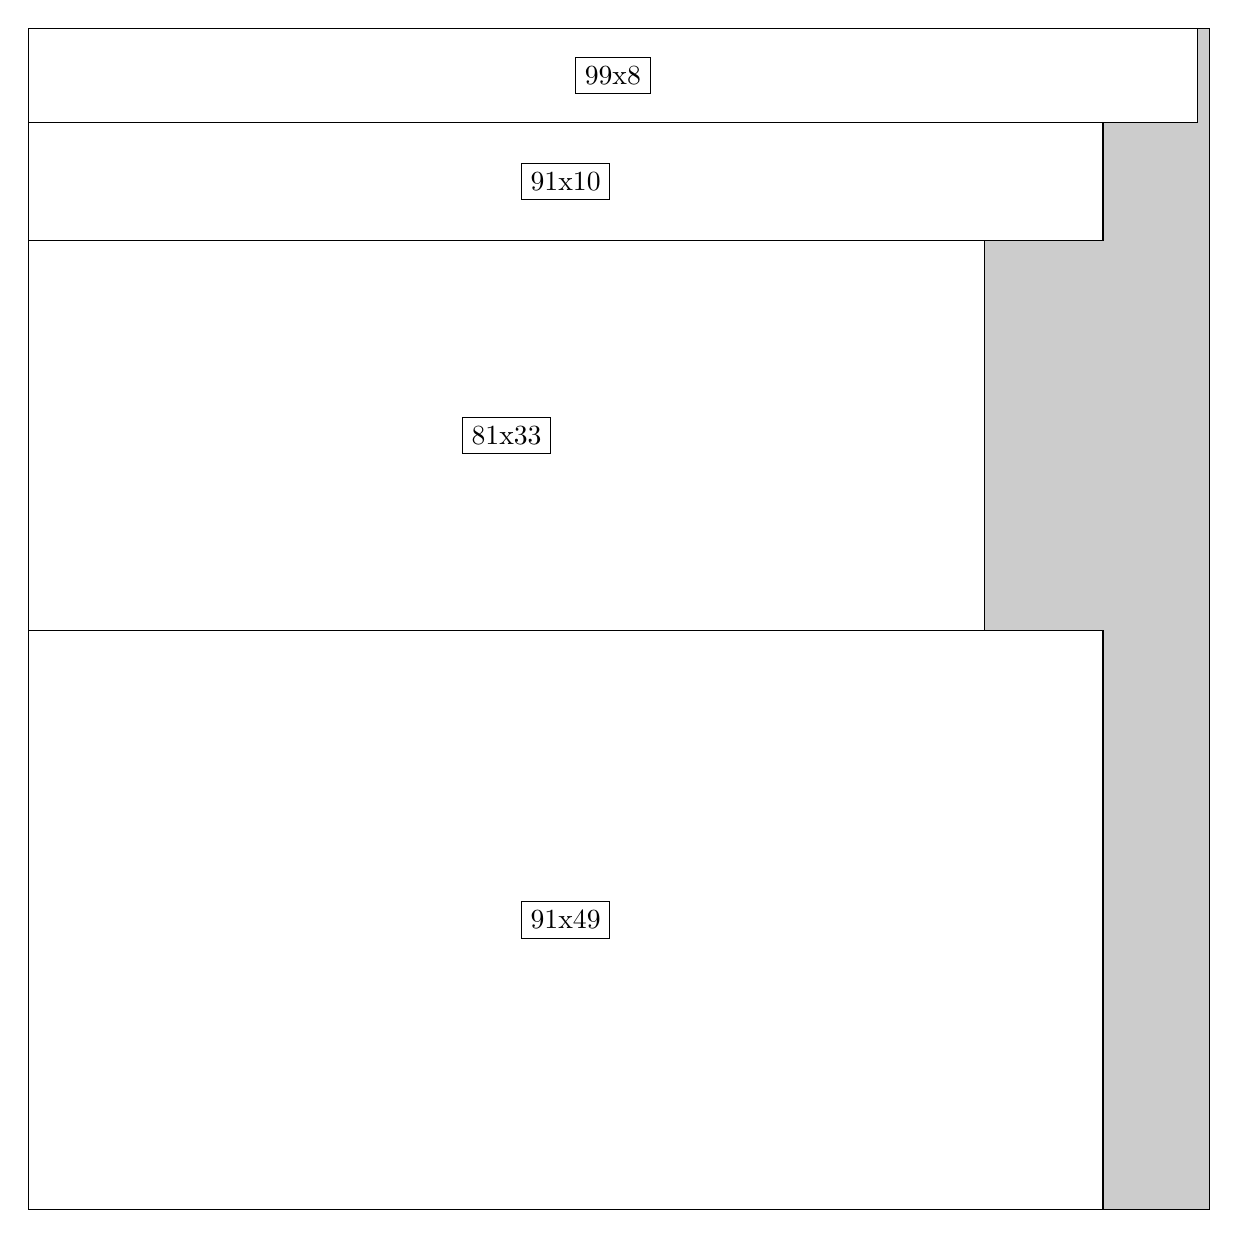
\begin{tikzpicture}[shorten >=1pt,scale=1.0,every node/.style={scale=1.0},->]
\tikzstyle{vertex}=[circle,fill=black!25,minimum size=14pt,inner sep=0pt]
\filldraw[fill=gray!40!white, draw=black] (0,0) rectangle (15.0,15.0);
\foreach \name/\x/\y/\w/\h in {91x49/0.0/0.0/13.65/7.35,81x33/0.0/7.35/12.15/4.95,91x10/0.0/12.299999999999999/13.65/1.5,99x8/0.0/13.799999999999999/14.85/1.2}
\filldraw[fill=white!40!white, draw=black] (\x,\y) rectangle node[draw] (\name) {\name} ++(\w,\h);
\end{tikzpicture}


w =91 , h =49 , x =0 , y =0 , v =4459
\par
w =81 , h =33 , x =0 , y =49 , v =2673
\par
w =91 , h =10 , x =0 , y =82 , v =910
\par
w =99 , h =8 , x =0 , y =92 , v =792
\par
\newpage


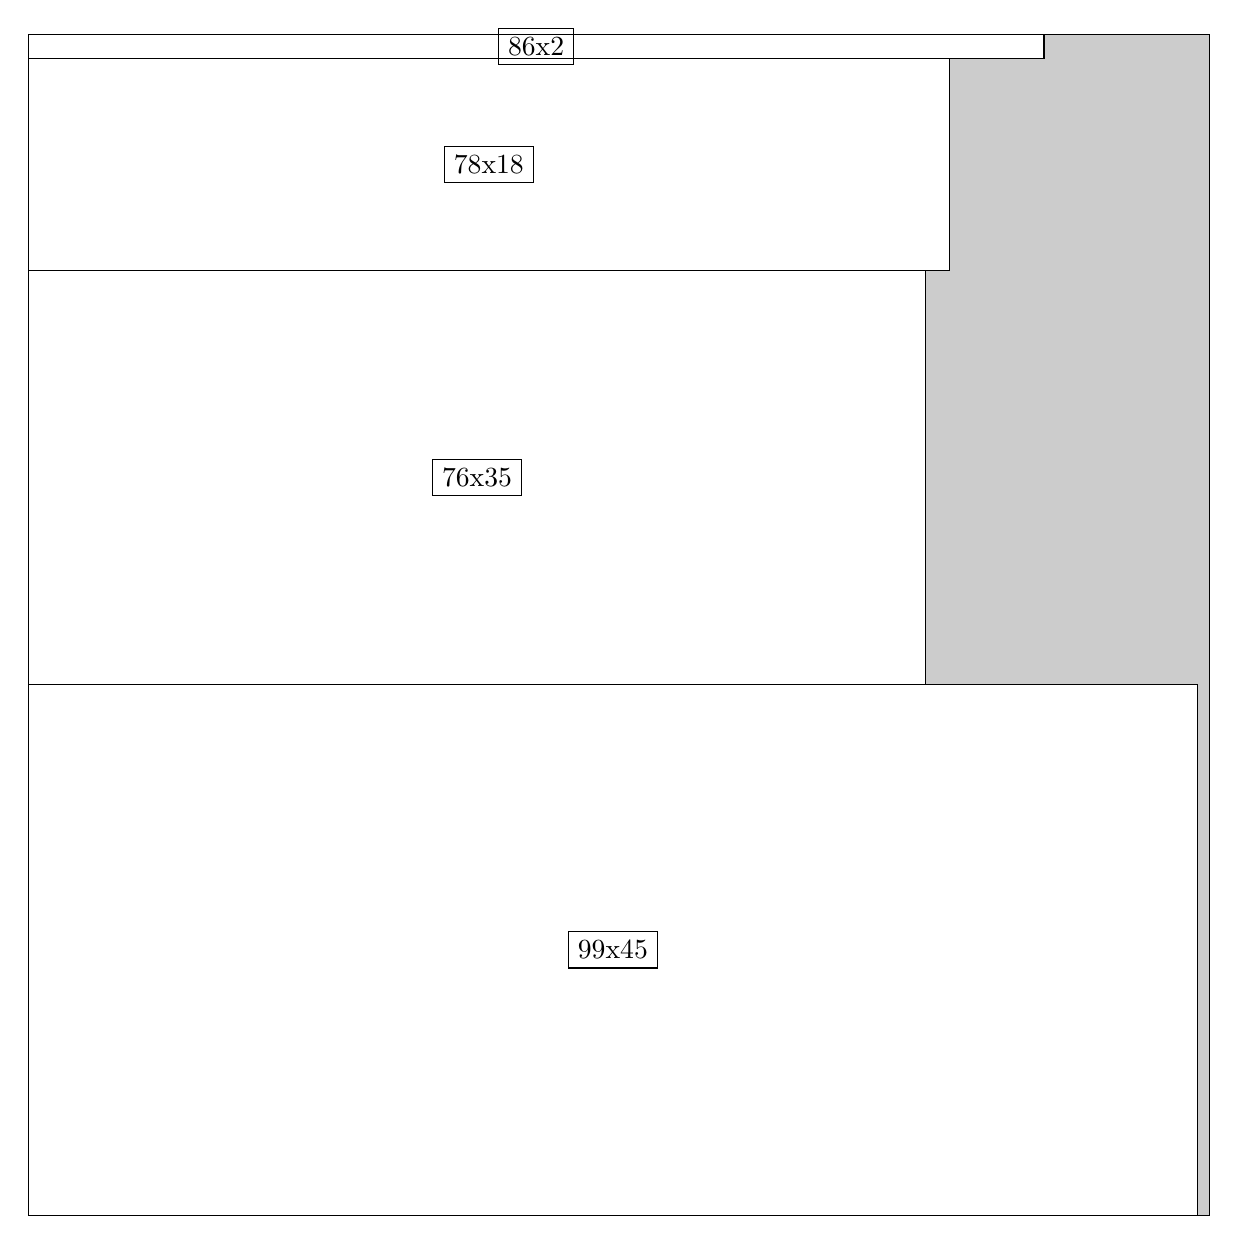
\begin{tikzpicture}[shorten >=1pt,scale=1.0,every node/.style={scale=1.0},->]
\tikzstyle{vertex}=[circle,fill=black!25,minimum size=14pt,inner sep=0pt]
\filldraw[fill=gray!40!white, draw=black] (0,0) rectangle (15.0,15.0);
\foreach \name/\x/\y/\w/\h in {99x45/0.0/0.0/14.85/6.75,76x35/0.0/6.75/11.4/5.25,78x18/0.0/12.0/11.7/2.6999999999999997,86x2/0.0/14.7/12.9/0.3}
\filldraw[fill=white!40!white, draw=black] (\x,\y) rectangle node[draw] (\name) {\name} ++(\w,\h);
\end{tikzpicture}


w =99 , h =45 , x =0 , y =0 , v =4455
\par
w =76 , h =35 , x =0 , y =45 , v =2660
\par
w =78 , h =18 , x =0 , y =80 , v =1404
\par
w =86 , h =2 , x =0 , y =98 , v =172
\par
\newpage


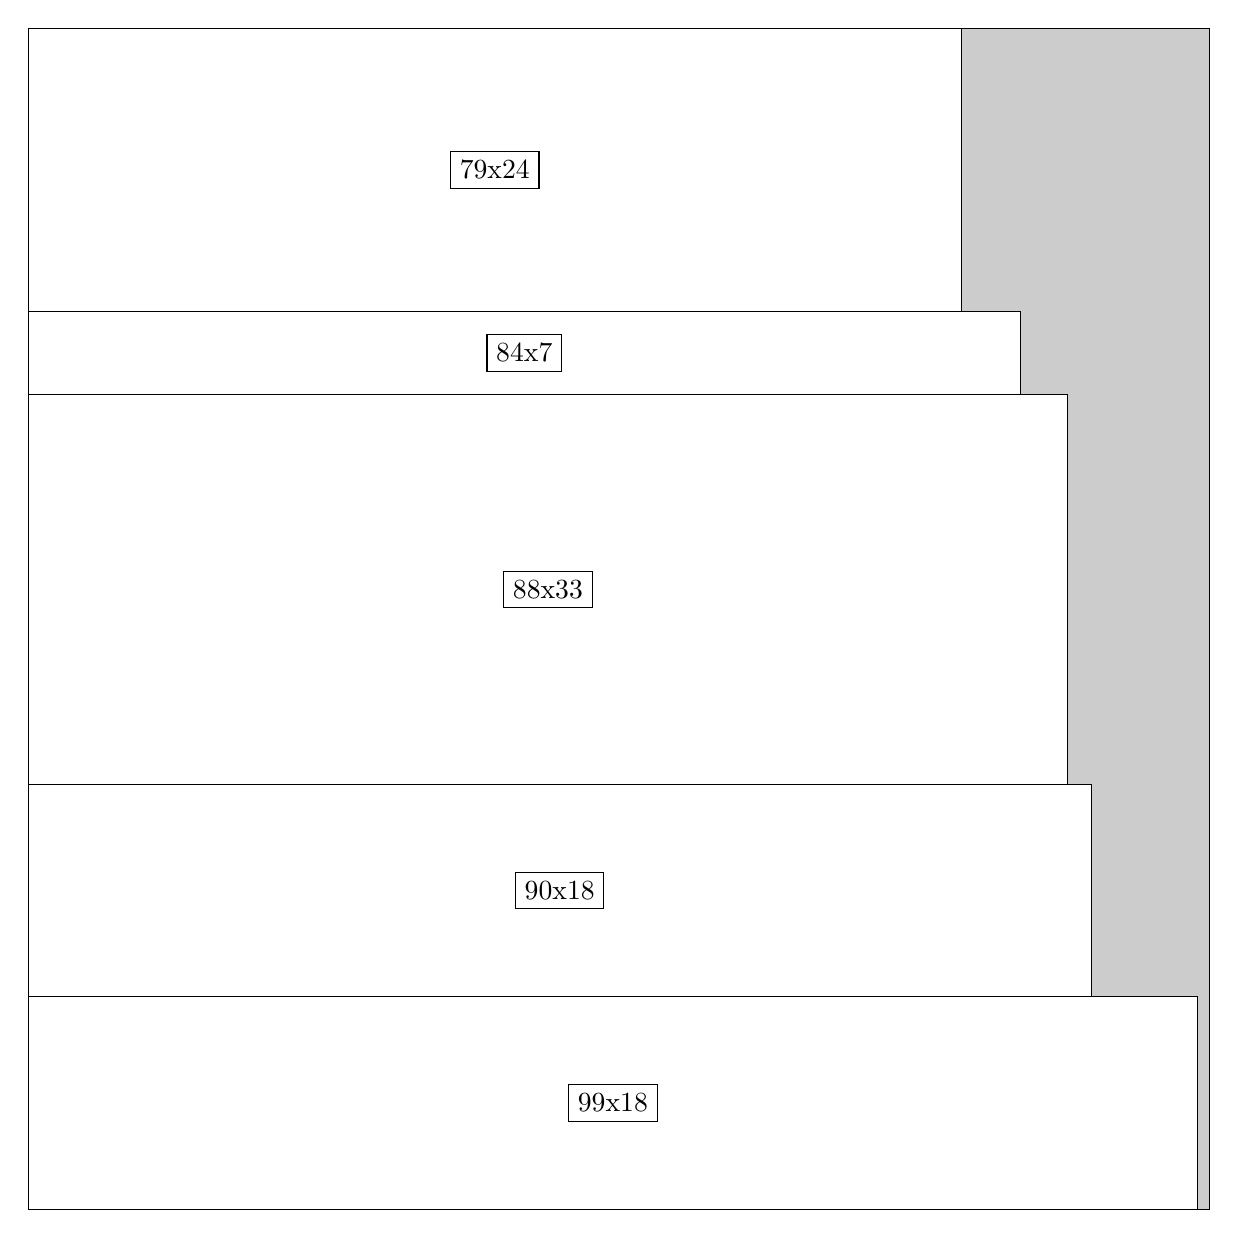
\begin{tikzpicture}[shorten >=1pt,scale=1.0,every node/.style={scale=1.0},->]
\tikzstyle{vertex}=[circle,fill=black!25,minimum size=14pt,inner sep=0pt]
\filldraw[fill=gray!40!white, draw=black] (0,0) rectangle (15.0,15.0);
\foreach \name/\x/\y/\w/\h in {88x33/0.0/5.3999999999999995/13.2/4.95,79x24/0.0/11.4/11.85/3.5999999999999996,99x18/0.0/0.0/14.85/2.6999999999999997,90x18/0.0/2.6999999999999997/13.5/2.6999999999999997,84x7/0.0/10.35/12.6/1.05}
\filldraw[fill=white!40!white, draw=black] (\x,\y) rectangle node[draw] (\name) {\name} ++(\w,\h);
\end{tikzpicture}


w =88 , h =33 , x =0 , y =36 , v =2904
\par
w =79 , h =24 , x =0 , y =76 , v =1896
\par
w =99 , h =18 , x =0 , y =0 , v =1782
\par
w =90 , h =18 , x =0 , y =18 , v =1620
\par
w =84 , h =7 , x =0 , y =69 , v =588
\par
\newpage


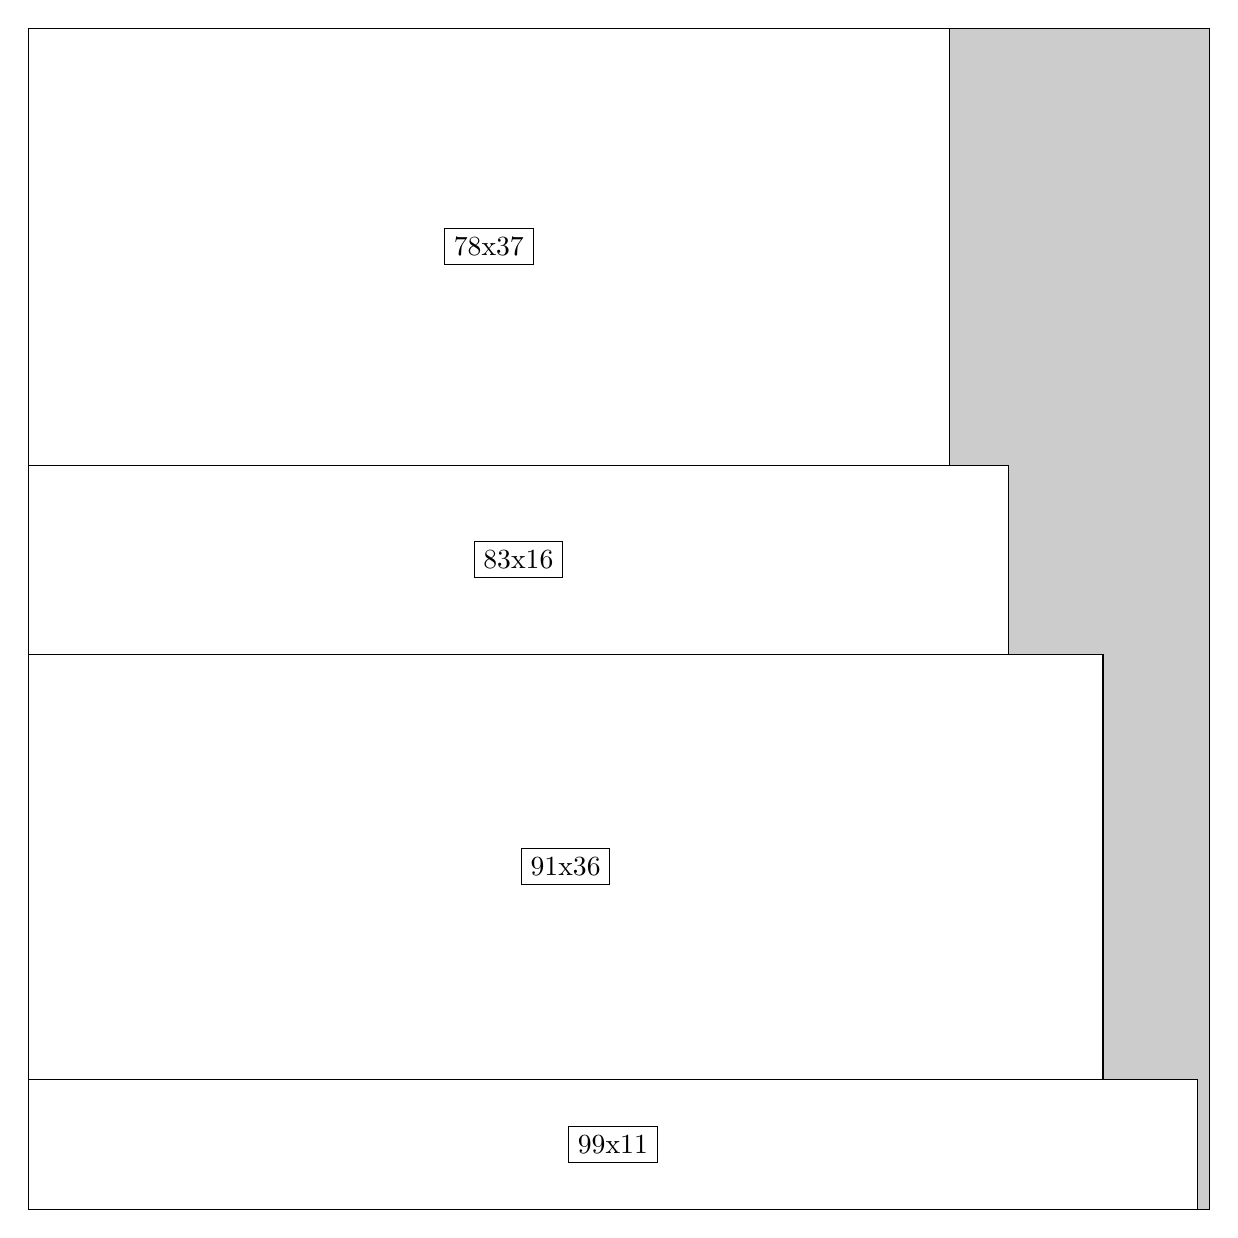
\begin{tikzpicture}[shorten >=1pt,scale=1.0,every node/.style={scale=1.0},->]
\tikzstyle{vertex}=[circle,fill=black!25,minimum size=14pt,inner sep=0pt]
\filldraw[fill=gray!40!white, draw=black] (0,0) rectangle (15.0,15.0);
\foreach \name/\x/\y/\w/\h in {91x36/0.0/1.65/13.65/5.3999999999999995,78x37/0.0/9.45/11.7/5.55,83x16/0.0/7.05/12.45/2.4,99x11/0.0/0.0/14.85/1.65}
\filldraw[fill=white!40!white, draw=black] (\x,\y) rectangle node[draw] (\name) {\name} ++(\w,\h);
\end{tikzpicture}


w =91 , h =36 , x =0 , y =11 , v =3276
\par
w =78 , h =37 , x =0 , y =63 , v =2886
\par
w =83 , h =16 , x =0 , y =47 , v =1328
\par
w =99 , h =11 , x =0 , y =0 , v =1089
\par
\newpage


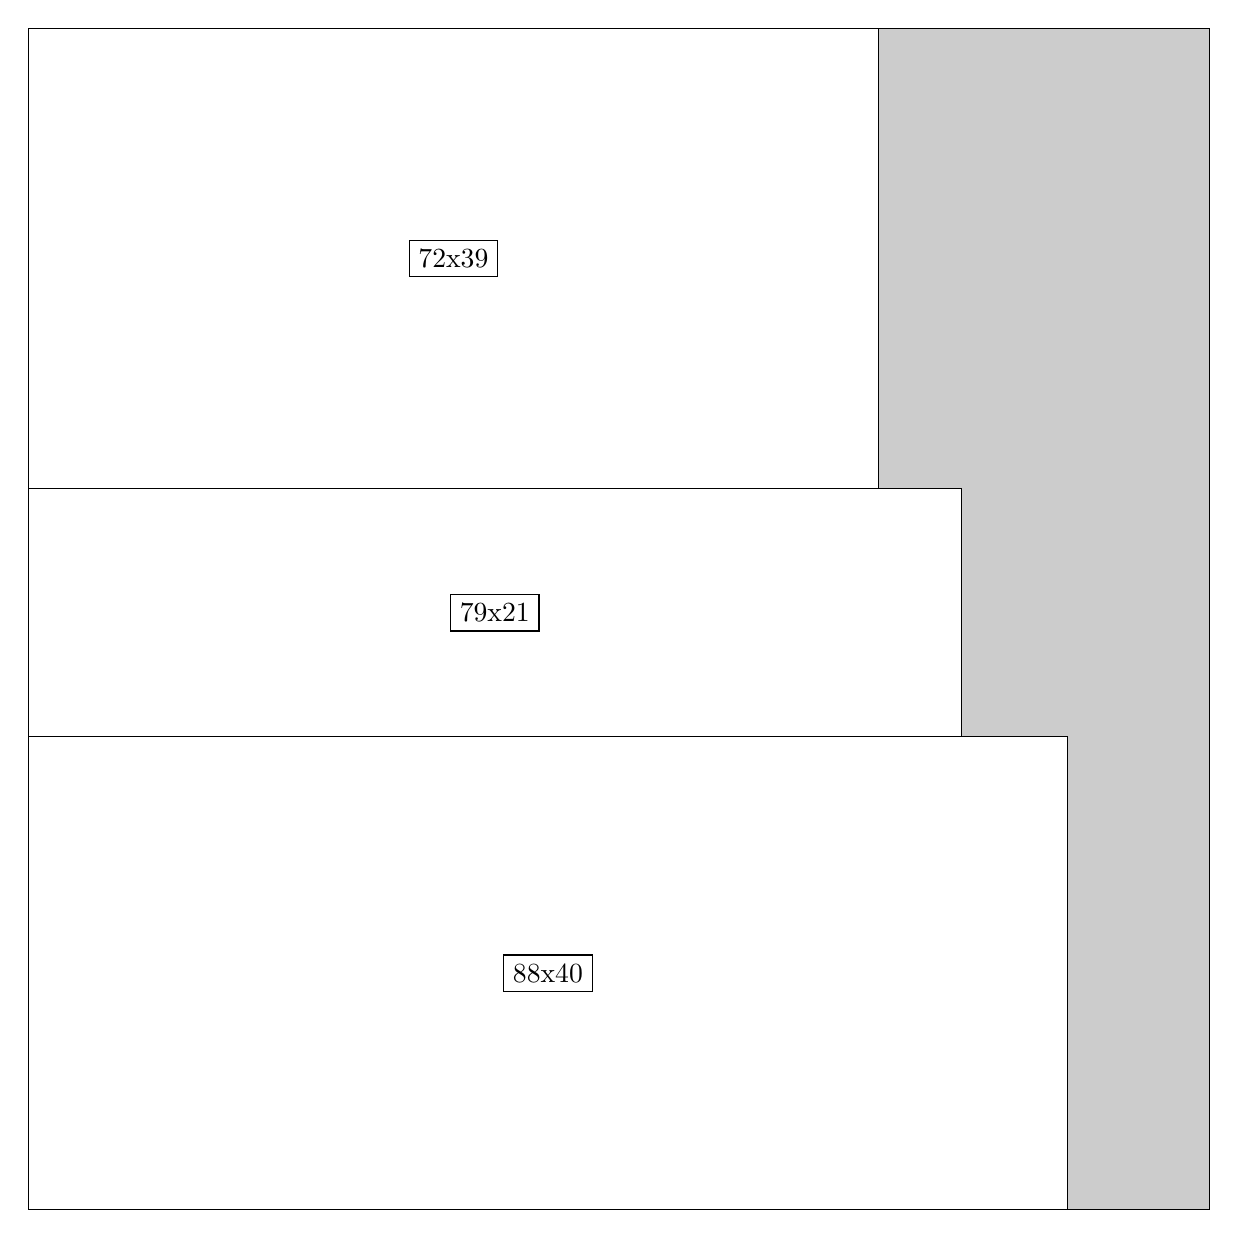
\begin{tikzpicture}[shorten >=1pt,scale=1.0,every node/.style={scale=1.0},->]
\tikzstyle{vertex}=[circle,fill=black!25,minimum size=14pt,inner sep=0pt]
\filldraw[fill=gray!40!white, draw=black] (0,0) rectangle (15.0,15.0);
\foreach \name/\x/\y/\w/\h in {88x40/0.0/0.0/13.2/6.0,72x39/0.0/9.15/10.799999999999999/5.85,79x21/0.0/6.0/11.85/3.15}
\filldraw[fill=white!40!white, draw=black] (\x,\y) rectangle node[draw] (\name) {\name} ++(\w,\h);
\end{tikzpicture}


w =88 , h =40 , x =0 , y =0 , v =3520
\par
w =72 , h =39 , x =0 , y =61 , v =2808
\par
w =79 , h =21 , x =0 , y =40 , v =1659
\par
\newpage


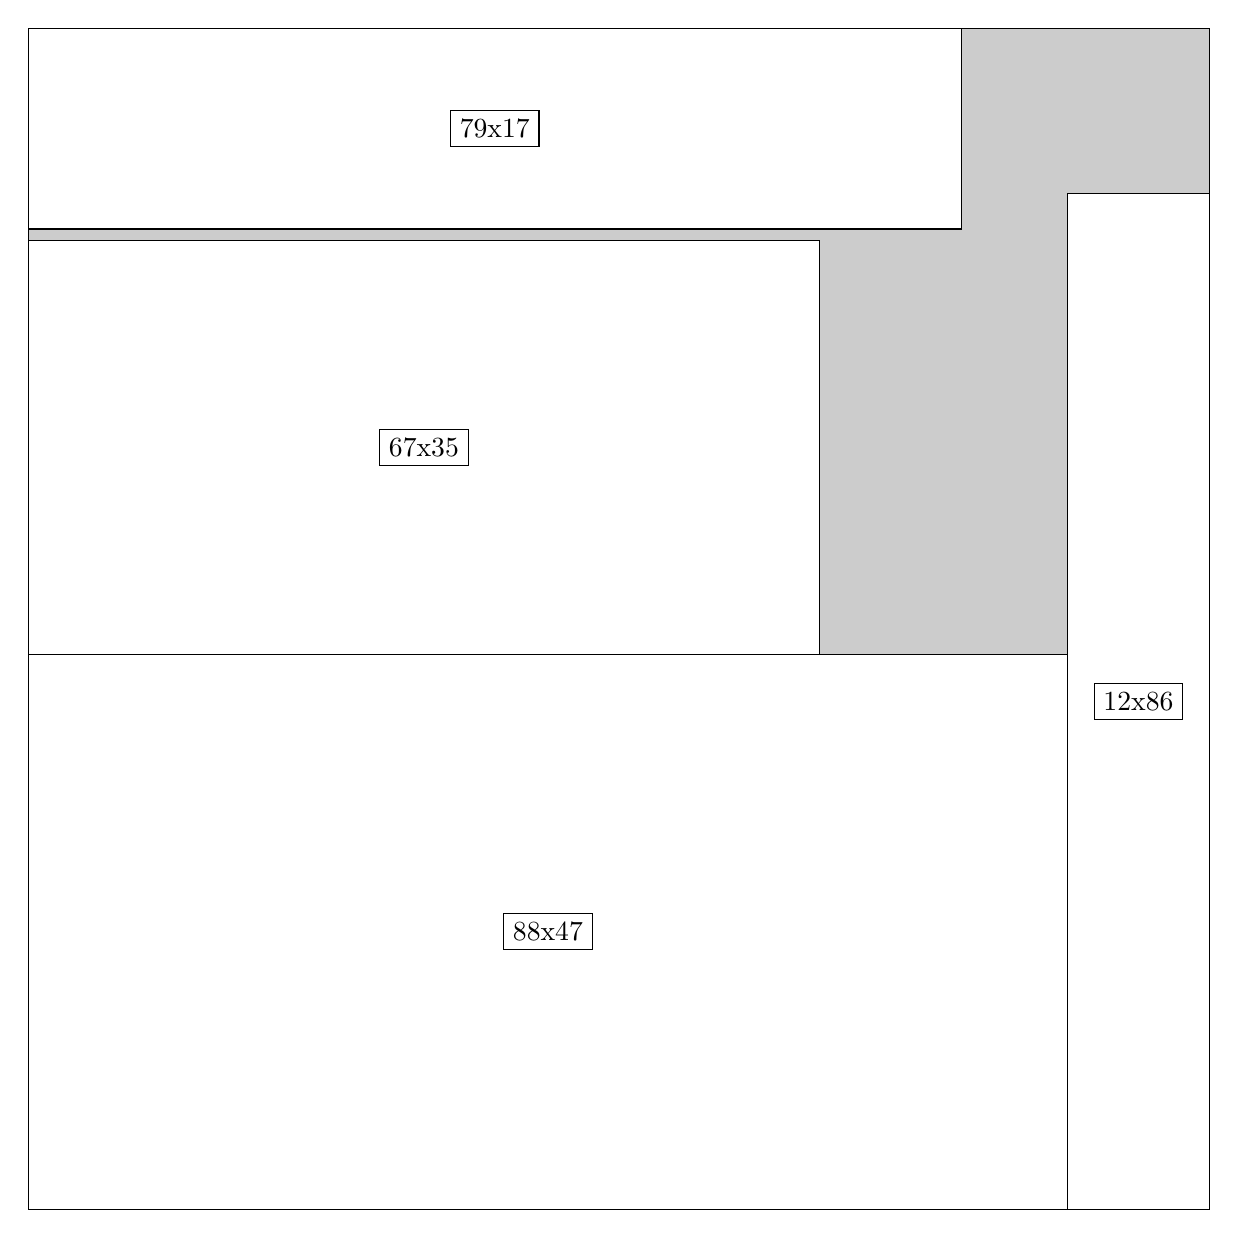
\begin{tikzpicture}[shorten >=1pt,scale=1.0,every node/.style={scale=1.0},->]
\tikzstyle{vertex}=[circle,fill=black!25,minimum size=14pt,inner sep=0pt]
\filldraw[fill=gray!40!white, draw=black] (0,0) rectangle (15.0,15.0);
\foreach \name/\x/\y/\w/\h in {88x47/0.0/0.0/13.2/7.05,67x35/0.0/7.05/10.049999999999999/5.25,79x17/0.0/12.45/11.85/2.55,12x86/13.2/0.0/1.7999999999999998/12.9}
\filldraw[fill=white!40!white, draw=black] (\x,\y) rectangle node[draw] (\name) {\name} ++(\w,\h);
\end{tikzpicture}


w =88 , h =47 , x =0 , y =0 , v =4136
\par
w =67 , h =35 , x =0 , y =47 , v =2345
\par
w =79 , h =17 , x =0 , y =83 , v =1343
\par
w =12 , h =86 , x =88 , y =0 , v =1032
\par
\newpage


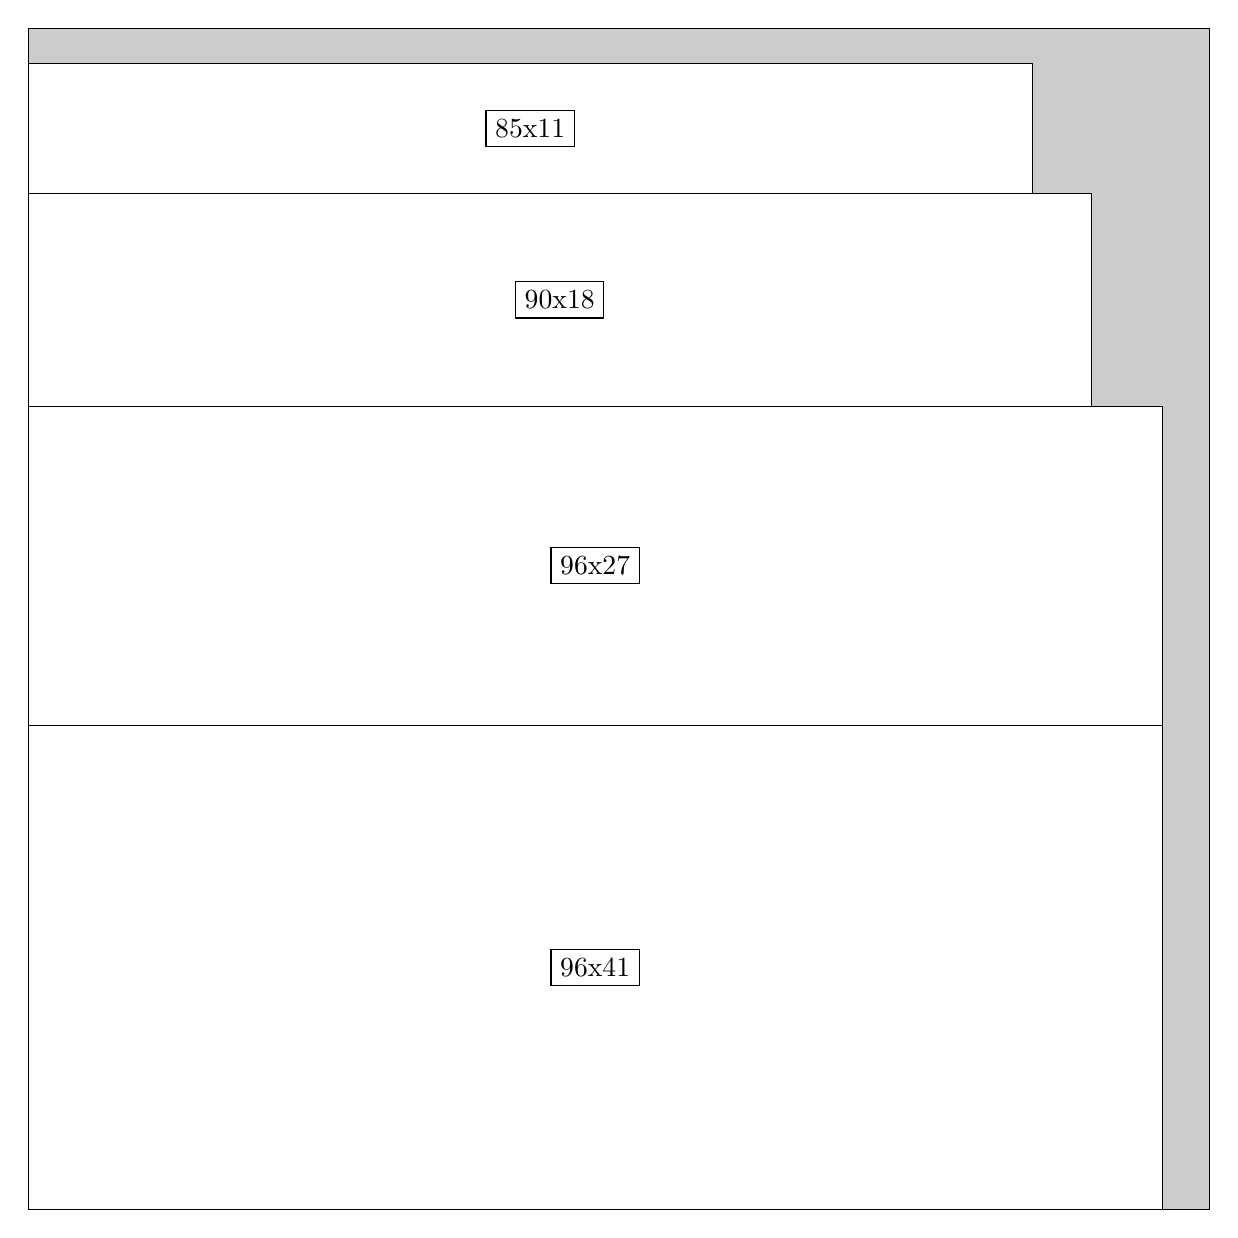
\begin{tikzpicture}[shorten >=1pt,scale=1.0,every node/.style={scale=1.0},->]
\tikzstyle{vertex}=[circle,fill=black!25,minimum size=14pt,inner sep=0pt]
\filldraw[fill=gray!40!white, draw=black] (0,0) rectangle (15.0,15.0);
\foreach \name/\x/\y/\w/\h in {96x41/0.0/0.0/14.399999999999999/6.1499999999999995,96x27/0.0/6.1499999999999995/14.399999999999999/4.05,90x18/0.0/10.2/13.5/2.6999999999999997,85x11/0.0/12.9/12.75/1.65}
\filldraw[fill=white!40!white, draw=black] (\x,\y) rectangle node[draw] (\name) {\name} ++(\w,\h);
\end{tikzpicture}


w =96 , h =41 , x =0 , y =0 , v =3936
\par
w =96 , h =27 , x =0 , y =41 , v =2592
\par
w =90 , h =18 , x =0 , y =68 , v =1620
\par
w =85 , h =11 , x =0 , y =86 , v =935
\par
\newpage


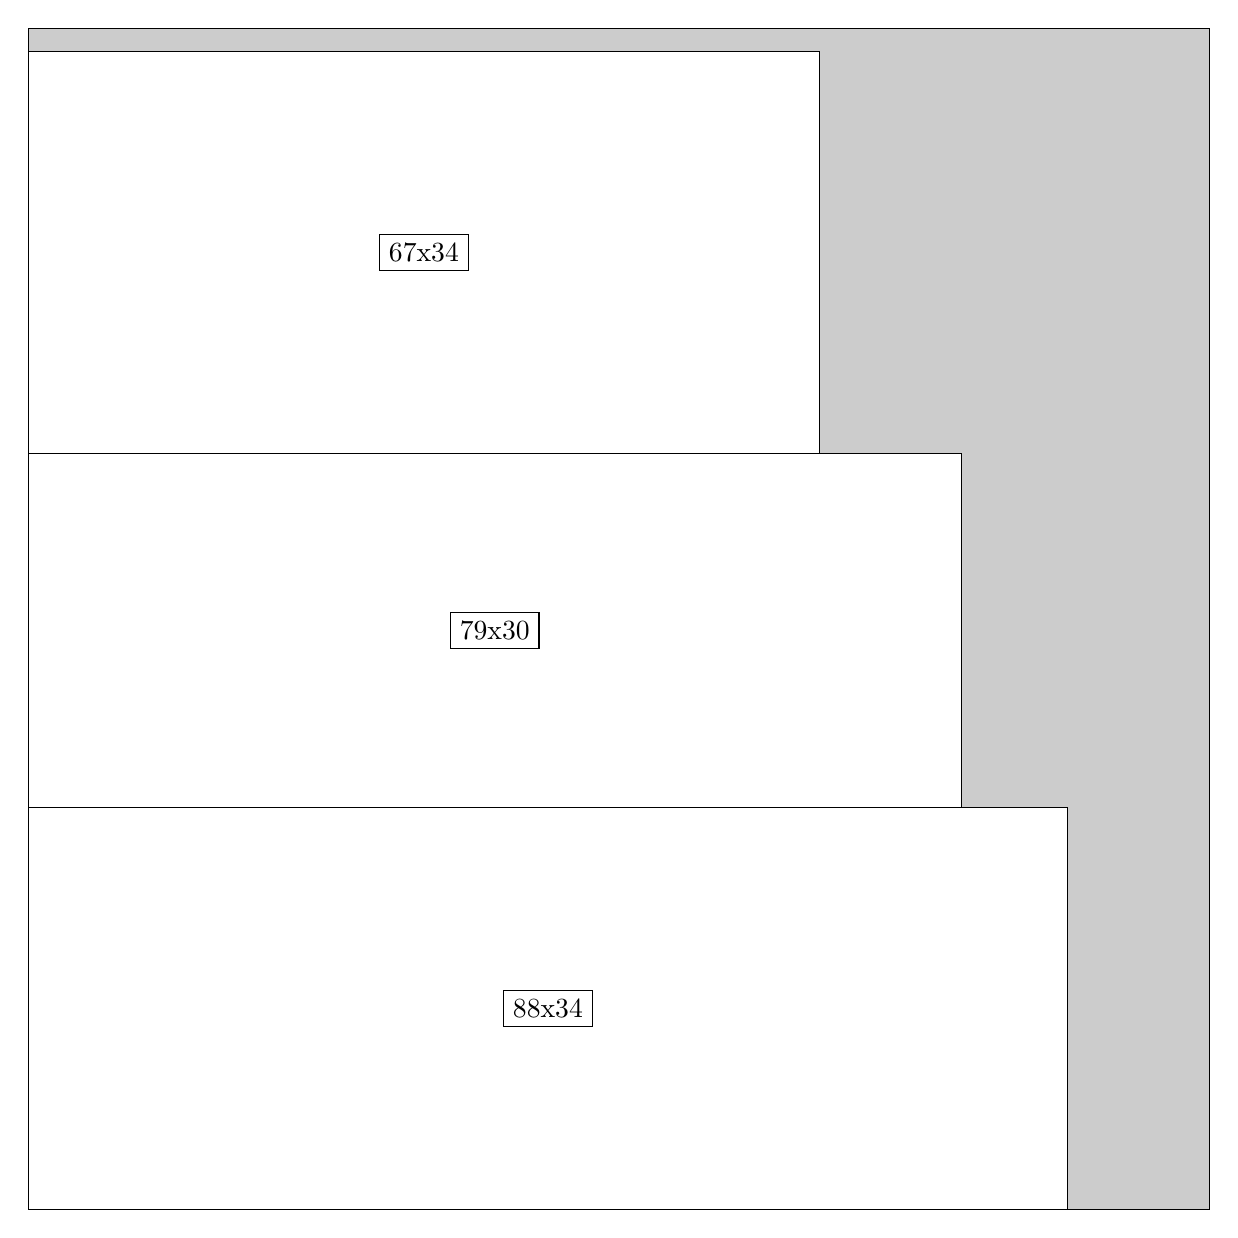
\begin{tikzpicture}[shorten >=1pt,scale=1.0,every node/.style={scale=1.0},->]
\tikzstyle{vertex}=[circle,fill=black!25,minimum size=14pt,inner sep=0pt]
\filldraw[fill=gray!40!white, draw=black] (0,0) rectangle (15.0,15.0);
\foreach \name/\x/\y/\w/\h in {88x34/0.0/0.0/13.2/5.1,79x30/0.0/5.1/11.85/4.5,67x34/0.0/9.6/10.049999999999999/5.1}
\filldraw[fill=white!40!white, draw=black] (\x,\y) rectangle node[draw] (\name) {\name} ++(\w,\h);
\end{tikzpicture}


w =88 , h =34 , x =0 , y =0 , v =2992
\par
w =79 , h =30 , x =0 , y =34 , v =2370
\par
w =67 , h =34 , x =0 , y =64 , v =2278
\par
\newpage


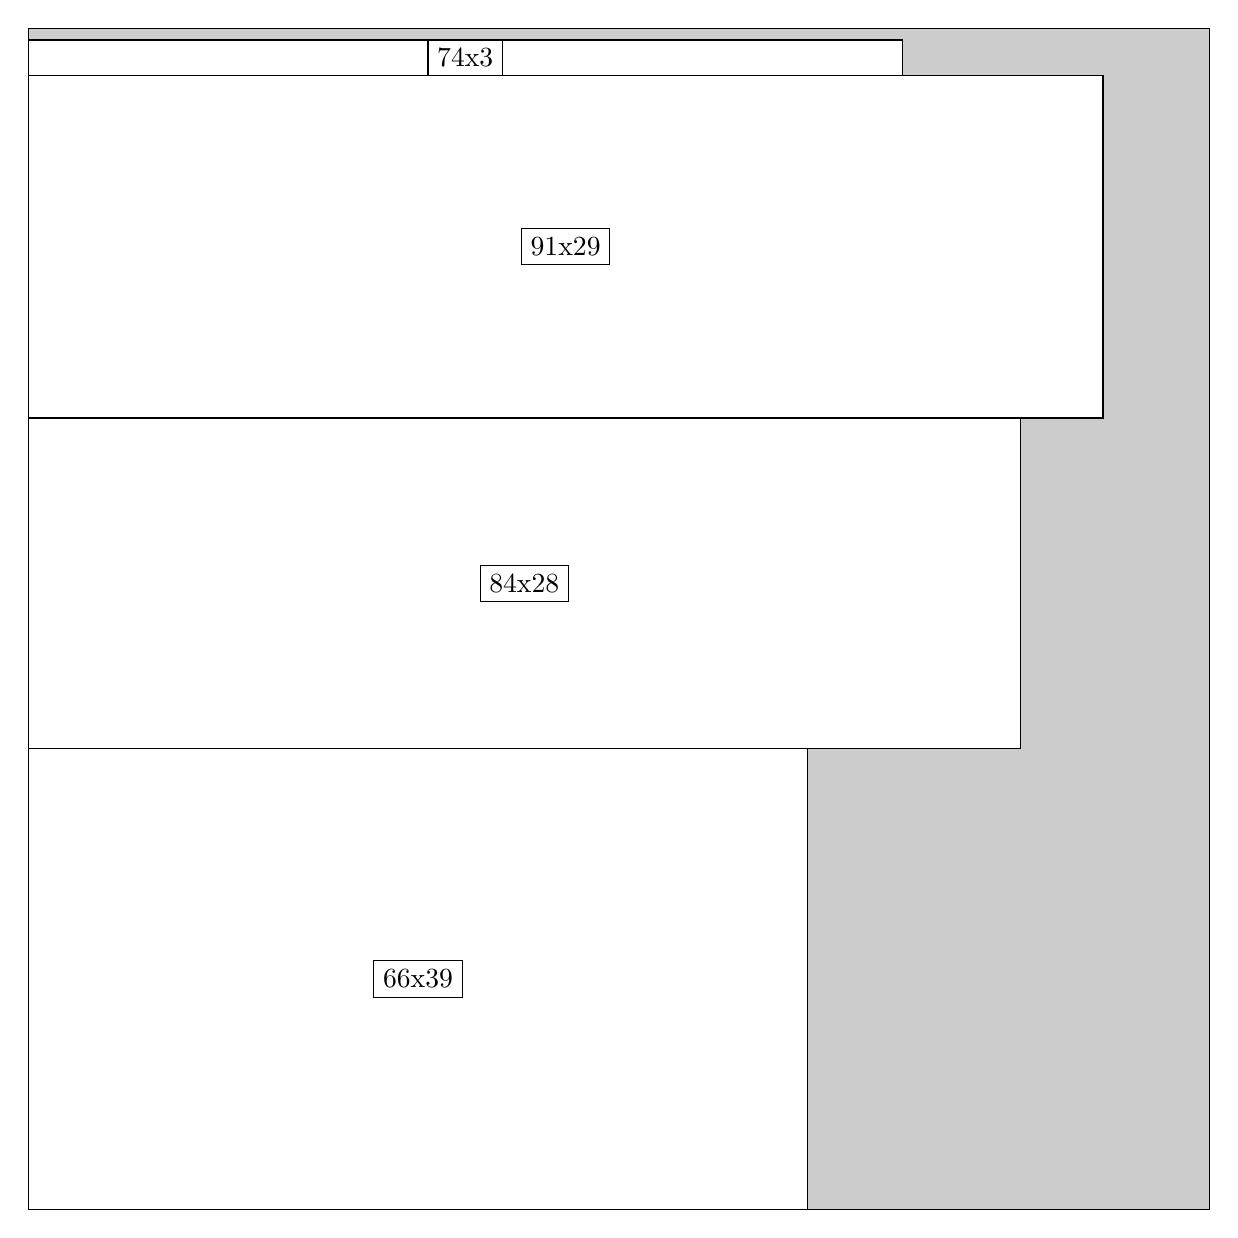
\begin{tikzpicture}[shorten >=1pt,scale=1.0,every node/.style={scale=1.0},->]
\tikzstyle{vertex}=[circle,fill=black!25,minimum size=14pt,inner sep=0pt]
\filldraw[fill=gray!40!white, draw=black] (0,0) rectangle (15.0,15.0);
\foreach \name/\x/\y/\w/\h in {91x29/0.0/10.049999999999999/13.65/4.35,84x28/0.0/5.85/12.6/4.2,66x39/0.0/0.0/9.9/5.85,74x3/0.0/14.399999999999999/11.1/0.44999999999999996}
\filldraw[fill=white!40!white, draw=black] (\x,\y) rectangle node[draw] (\name) {\name} ++(\w,\h);
\end{tikzpicture}


w =91 , h =29 , x =0 , y =67 , v =2639
\par
w =84 , h =28 , x =0 , y =39 , v =2352
\par
w =66 , h =39 , x =0 , y =0 , v =2574
\par
w =74 , h =3 , x =0 , y =96 , v =222
\par
\newpage


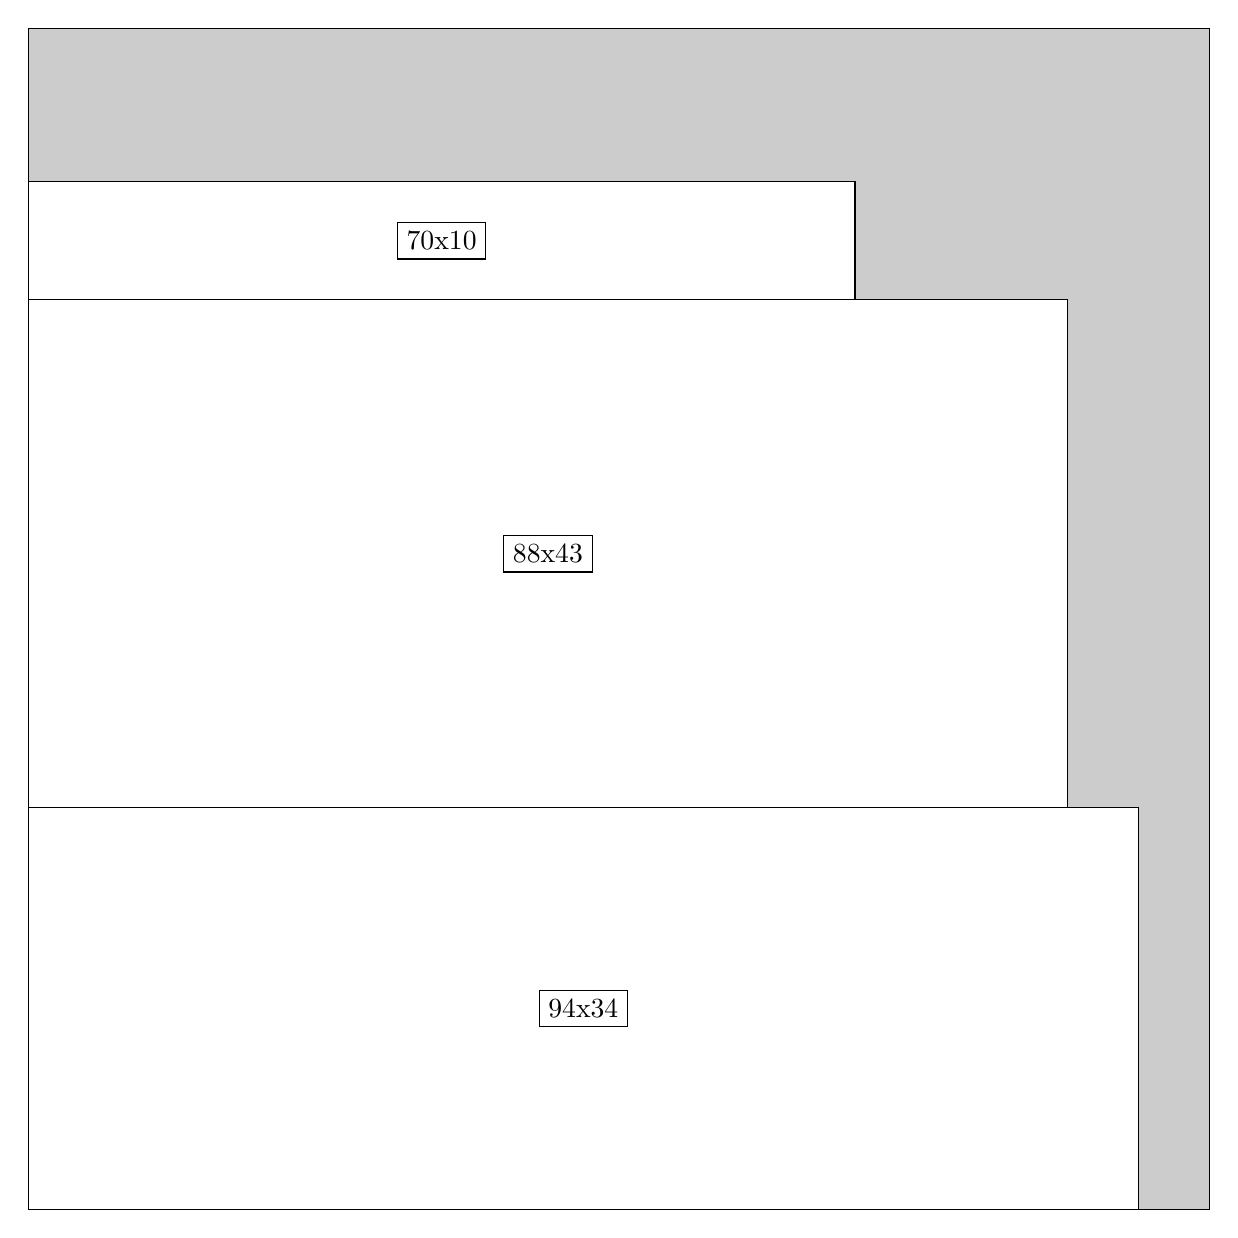
\begin{tikzpicture}[shorten >=1pt,scale=1.0,every node/.style={scale=1.0},->]
\tikzstyle{vertex}=[circle,fill=black!25,minimum size=14pt,inner sep=0pt]
\filldraw[fill=gray!40!white, draw=black] (0,0) rectangle (15.0,15.0);
\foreach \name/\x/\y/\w/\h in {94x34/0.0/0.0/14.1/5.1,88x43/0.0/5.1/13.2/6.45,70x10/0.0/11.549999999999999/10.5/1.5}
\filldraw[fill=white!40!white, draw=black] (\x,\y) rectangle node[draw] (\name) {\name} ++(\w,\h);
\end{tikzpicture}


w =94 , h =34 , x =0 , y =0 , v =3196
\par
w =88 , h =43 , x =0 , y =34 , v =3784
\par
w =70 , h =10 , x =0 , y =77 , v =700
\par
\newpage


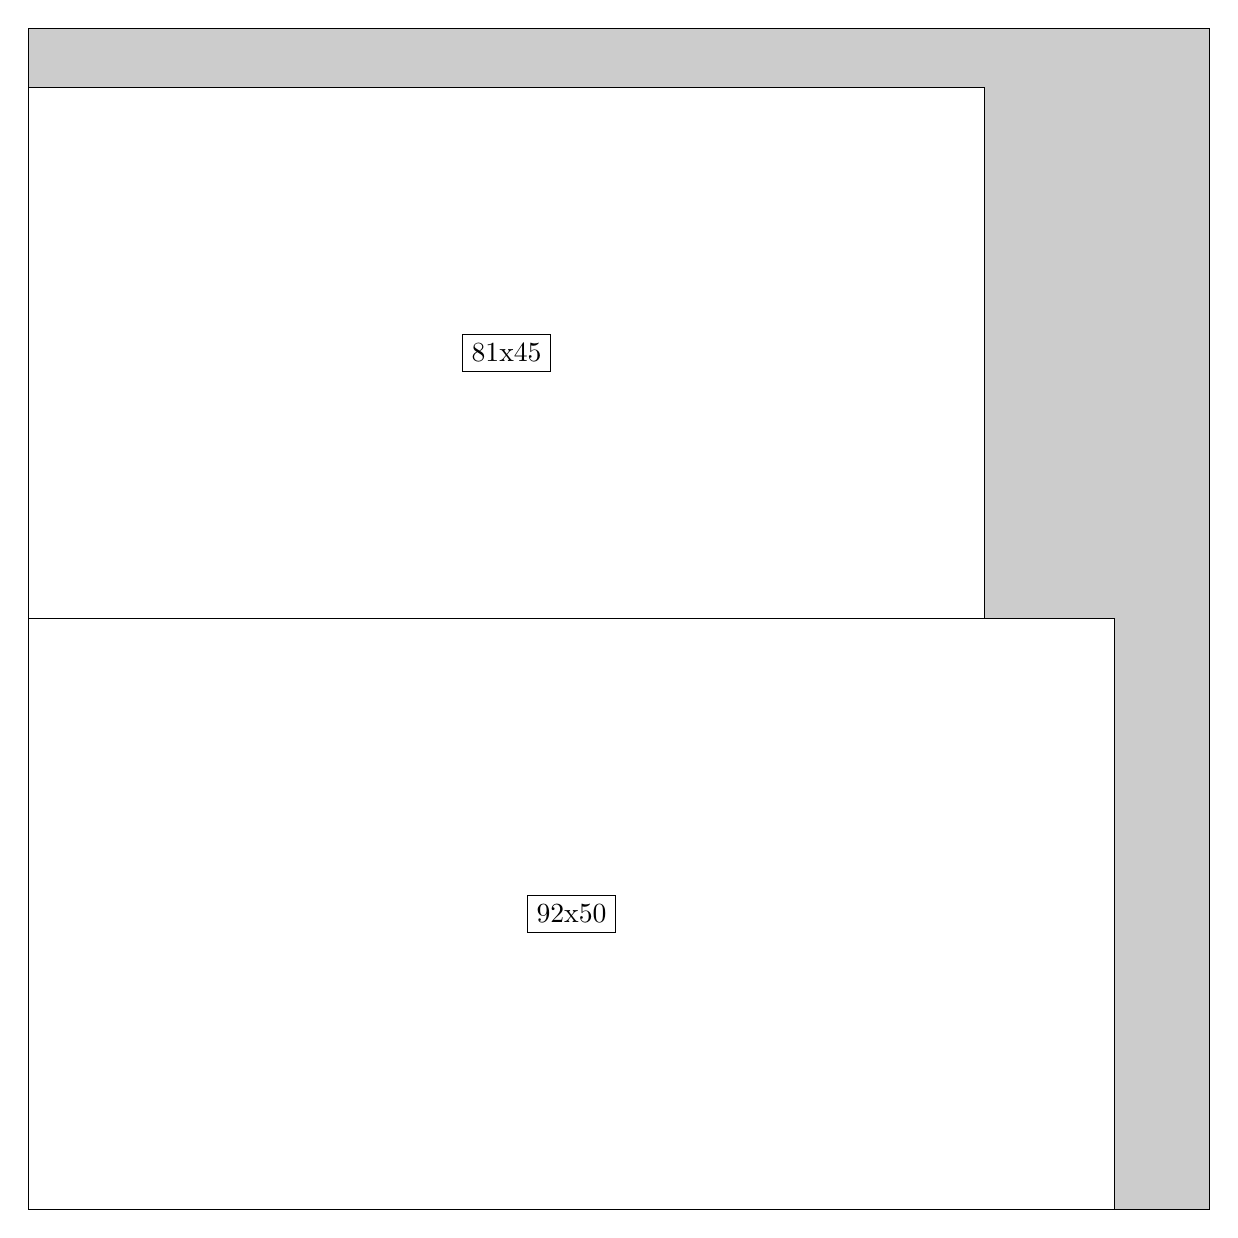
\begin{tikzpicture}[shorten >=1pt,scale=1.0,every node/.style={scale=1.0},->]
\tikzstyle{vertex}=[circle,fill=black!25,minimum size=14pt,inner sep=0pt]
\filldraw[fill=gray!40!white, draw=black] (0,0) rectangle (15.0,15.0);
\foreach \name/\x/\y/\w/\h in {92x50/0.0/0.0/13.799999999999999/7.5,81x45/0.0/7.5/12.15/6.75}
\filldraw[fill=white!40!white, draw=black] (\x,\y) rectangle node[draw] (\name) {\name} ++(\w,\h);
\end{tikzpicture}


w =92 , h =50 , x =0 , y =0 , v =4600
\par
w =81 , h =45 , x =0 , y =50 , v =3645
\par
\newpage


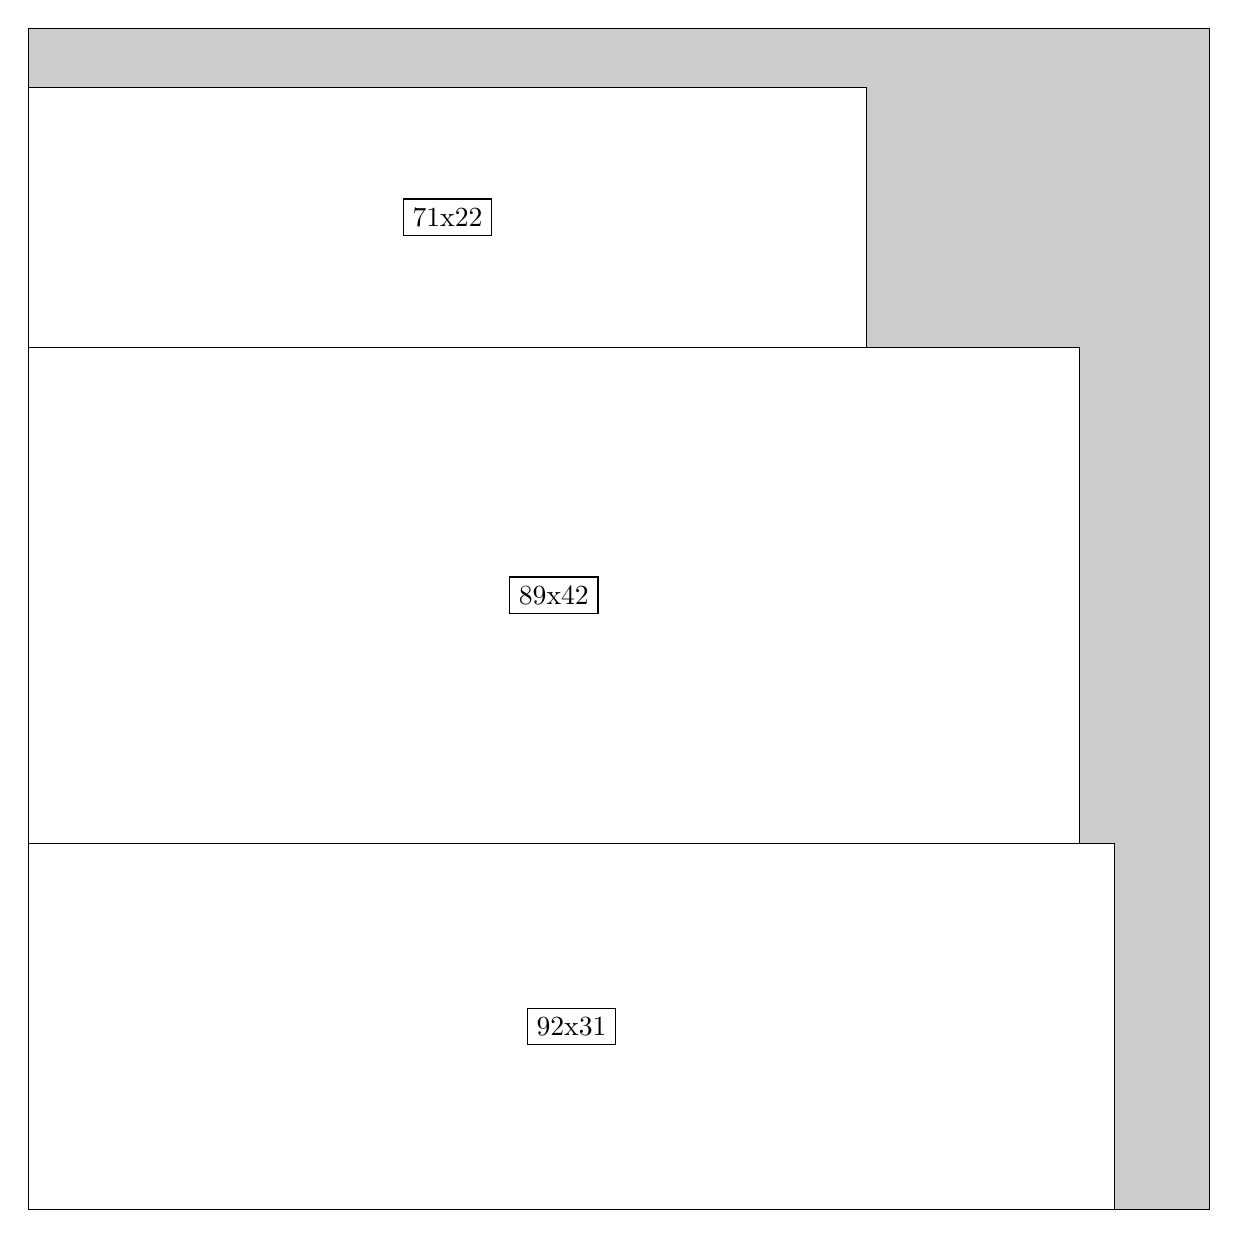
\begin{tikzpicture}[shorten >=1pt,scale=1.0,every node/.style={scale=1.0},->]
\tikzstyle{vertex}=[circle,fill=black!25,minimum size=14pt,inner sep=0pt]
\filldraw[fill=gray!40!white, draw=black] (0,0) rectangle (15.0,15.0);
\foreach \name/\x/\y/\w/\h in {89x42/0.0/4.6499999999999995/13.35/6.3,92x31/0.0/0.0/13.799999999999999/4.6499999999999995,71x22/0.0/10.95/10.65/3.3}
\filldraw[fill=white!40!white, draw=black] (\x,\y) rectangle node[draw] (\name) {\name} ++(\w,\h);
\end{tikzpicture}


w =89 , h =42 , x =0 , y =31 , v =3738
\par
w =92 , h =31 , x =0 , y =0 , v =2852
\par
w =71 , h =22 , x =0 , y =73 , v =1562
\par
\newpage


\end{document}